\documentclass[10pt,journal,compsoc]{IEEEtran}



\ifCLASSOPTIONcompsoc
  \usepackage[nocompress]{cite}
\else
  \usepackage{cite}
\fi

\usepackage{times}
\usepackage{epsfig}
\usepackage{graphicx}
\usepackage{amsmath}
\usepackage{amssymb}

\usepackage[dvipsnames]{xcolor}
\usepackage{booktabs}
\usepackage{multirow}
\usepackage{fixmath}
\usepackage{subcaption}
\usepackage{float}
\usepackage{xspace}
\usepackage{comment}
\usepackage{hyperref}
\usepackage[normalem]{ulem}
\usepackage[ruled]{algorithm2e}

\newcommand{\sign}{\mbox{sign}}
\newcommand{\relu}{\mbox{ReLU}}
\newcommand{\Var}{\mathrm{Var}}

\newcommand\blfootnote[1]{%
  \begingroup
  \renewcommand\thefootnote{}\footnote{#1}%
  \addtocounter{footnote}{-1}%
  \endgroup
}

\makeatletter
\newcommand\approxsim{\mathchoice
  {\@approxsim {\displaystyle}      {1ex} }
  {\@approxsim {\textstyle}         {1ex} }
  {\@approxsim {\scriptstyle}       {.7ex}}
  {\@approxsim {\scriptscriptstyle} {.5ex}}}
\newcommand\@approxsim[2]{%
  \mathrel{%
    \ooalign{%
      $\m@th#1\sim$\cr
      \hidewidth$\m@th#1.$\hidewidth\cr
      \hidewidth\raise #2 \hbox{$\m@th#1.$}\hidewidth\cr
    }%
  }%
}
\makeatother

\newcommand{\hl}[1]{\textcolor{YellowOrange}{#1}}

\newcommand{\enzo}[1]{\textcolor{blue}{Enzo: #1}}
\newcommand{\marco}[1]{\textcolor{cyan}{Marco: #1}}
\newcommand{\carlo}[1]{\textcolor{red}{#1 [Carlo]}}
\newcommand{\rephrase}[1]{\textcolor{teal}{\textbf{Rephrase:} #1}}
\newcommand{\improve}[1]{\textcolor{violet}{\textbf{Improve:} #1}}
\newcommand{\todo}[1]{\textcolor{purple}{\textbf{Todo:} #1}}
\newcommand{\proposal}[1]{\textcolor{olive}{\textbf{Proposal:} #1}}

\newcommand{\std}[1]{\scriptsize{$\pm$#1}}

\hyphenation{op-tical net-works semi-conduc-tor}


\begin{document}
\title{Unsupervised Learning of Unbiased Visual Representations}

\author{Carlo~Alberto~Barbano,
        Enzo~Tartaglione,~\IEEEmembership{Member,~IEEE},
        and~Marco~Grangetto,~\IEEEmembership{Senior~Member,~IEEE}%
\IEEEcompsocitemizethanks{\IEEEcompsocthanksitem C.A. Barbano is with the Department
of Computer Science, University of Turin, 10149, Italy, and with LTCI, Télécom Paris, Institut Polytechnique de Paris, 91120, France. %
E-mail: carlo.barbano@unito.it
\IEEEcompsocthanksitem E. Tartaglione is with LTCI, Télécom Paris, Institut Polytechnique de Paris, 91120, France. E-mail: enzo.tartaglione@telecom-paris.fr
\IEEEcompsocthanksitem M. Grangetto is with the Department
of Computer Science, University of Turin, 10149, Italy. E-mail: marco.grangetto@unito.it}%

\thanks{Preprint.}}




\markboth{Journal of \LaTeX\ Class Files,~Vol.~14, No.~8, August~2015}%
{Shell \MakeLowercase{\textit{et al.}}: Bare Demo of IEEEtran.cls for Computer Society Journals}









\IEEEtitleabstractindextext{%
\begin{abstract}
Deep neural networks are known for their inability to learn robust representations when biases exist in the dataset. This results in a poor generalization to unbiased datasets, as the predictions strongly rely on peripheral and confounding factors, which are erroneously learned by the network. Many existing works deal with this issue by either employing an explicit supervision on the bias attributes, or assuming prior knowledge about the bias.
In this work we study this problem in a more difficult scenario, in which no explicit annotation about the bias is available, and without any prior knowledge about its nature.
We propose a fully unsupervised debiasing framework, consisting of three steps: first, we exploit the natural preference for learning malignant biases, obtaining a bias-capturing model;
then, we perform a pseudo-labelling step to obtain bias labels; finally we employ state-of-the-art supervised debiasing techniques to obtain an unbiased model. We also propose a theoretical framework to assess the biasness of a model, and provide a detailed analysis on how biases affect the training of neural networks. We perform experiments on synthetic and real-world datasets, showing that our method achieves state-of-the-art performance in a variety of settings, sometimes even higher than fully supervised debiasing approaches.
\end{abstract}

\begin{IEEEkeywords}
Deep learning, Bias, Regularization, Unsupervised learning.
\end{IEEEkeywords}}


\maketitle


\IEEEdisplaynontitleabstractindextext



\IEEEpeerreviewmaketitle

\section{Introduction}



Motion mimicking aims to find a policy to generate control signals for recovering demonstrated motion trajectories, which plays a fundamental role in physics-based character animation, and also serves as a prerequisite for many applications such as control stylization and skill composition. 
Although tremendous progress in motion mimicking has been witnessed in recent years, existing methods~\citep{peng2018deepmimic, peng2021amp} mostly adopt reinforcement learning (RL) schemes, which require alternatively learning a reward function and a control policy.
Consequently, RL-based methods often take tens of hours or even days to imitate one single motion sequence, making their scalability notoriously challenging.
In addition, RL-based motion mimicking highly relies on the quality of its designed ~\citep{peng2018deepmimic} or learned~\citep{peng2021amp} reward functions, which further burdens its generalization for complex real-world applications.




Recently, differential physics simulator (DPS) has achieved impressive results in many research fields, such as robot control~\citep{xu2022accelerated} and graphics~\citep{li2022diffcloth}.
Specifically, DPS treats physics operators as differentiable computational graphs, and therefore gradients from objectives (\textit{i.e.}, rewards) can be directly propagated through the environment dynamics to control policy functions.
Instead of alternatively learning between reward functions and control policies, the control policy learning tasks can be resolved in a straightforward and efficient optimization manner with the help of DPS. 
However, despite their analytical environment gradients, optimization with DPS could easily get into local optima, particularly in contact-rich physical systems that often yield stiff and discontinuous gradients~\citep{freeman2021brax, suh2022does, zhong2022differentiable}. 
Besides, numerical gradients could also vanish/explode along the backward path for long trajectories.






In this work, we propose DiffMimic, a fast and stable motion mimicking method with the help of DPS.
Different from RL-based methods that require heavy reward engineering and poor sample efficiency, DiffMimic reformulates motion mimicking as a state matching problem, which could directly minimize the distance between a rollout trajectory generated by the current learning policy and the demonstrated trajectory.
Thanks to the differentiable DPS dynamics, gradients of the trajectory distance can be directly propagated to optimize the control policy.
As a result, DiffMimic could significantly improve the sample efficiency with the first-order gradients.

However, simply utilizing DPS could not guarantee global optimal solutions.
In particular, the rollout trajectory tends to gradually deviate from the expert demonstration and could produce a large accumulative error for long motion sequences, due to the distributional shift between the learning policy and expert policy.
To address these problems, we introduce the \textit{\ourmethod{}} training strategy, which randomly inserts reference states into the rollout trajectory as anchor states to guide the exploration of the policy. 
Empirically, \ourmethod{} gives a smoother gradient estimation, which significantly stabilizes the policy learning of DiffMimic.


To the best of our knowledge, DiffMimic is the first to utilize DPS for motion mimicking. We show that DiffMimic outperforms several commonly used RL-based methods for motion mimicking on a variety of tasks with high accuracy, stability, and efficiency. In particular, DiffMimic allows learning a challenging \textit{Backflip} motion in only 10 minutes on a single V100 GPU.
In addition, we release the DiffMimic simulator as a standard benchmark to encourage future research for motion mimicking.

\begin{figure}[t]
    \centering
    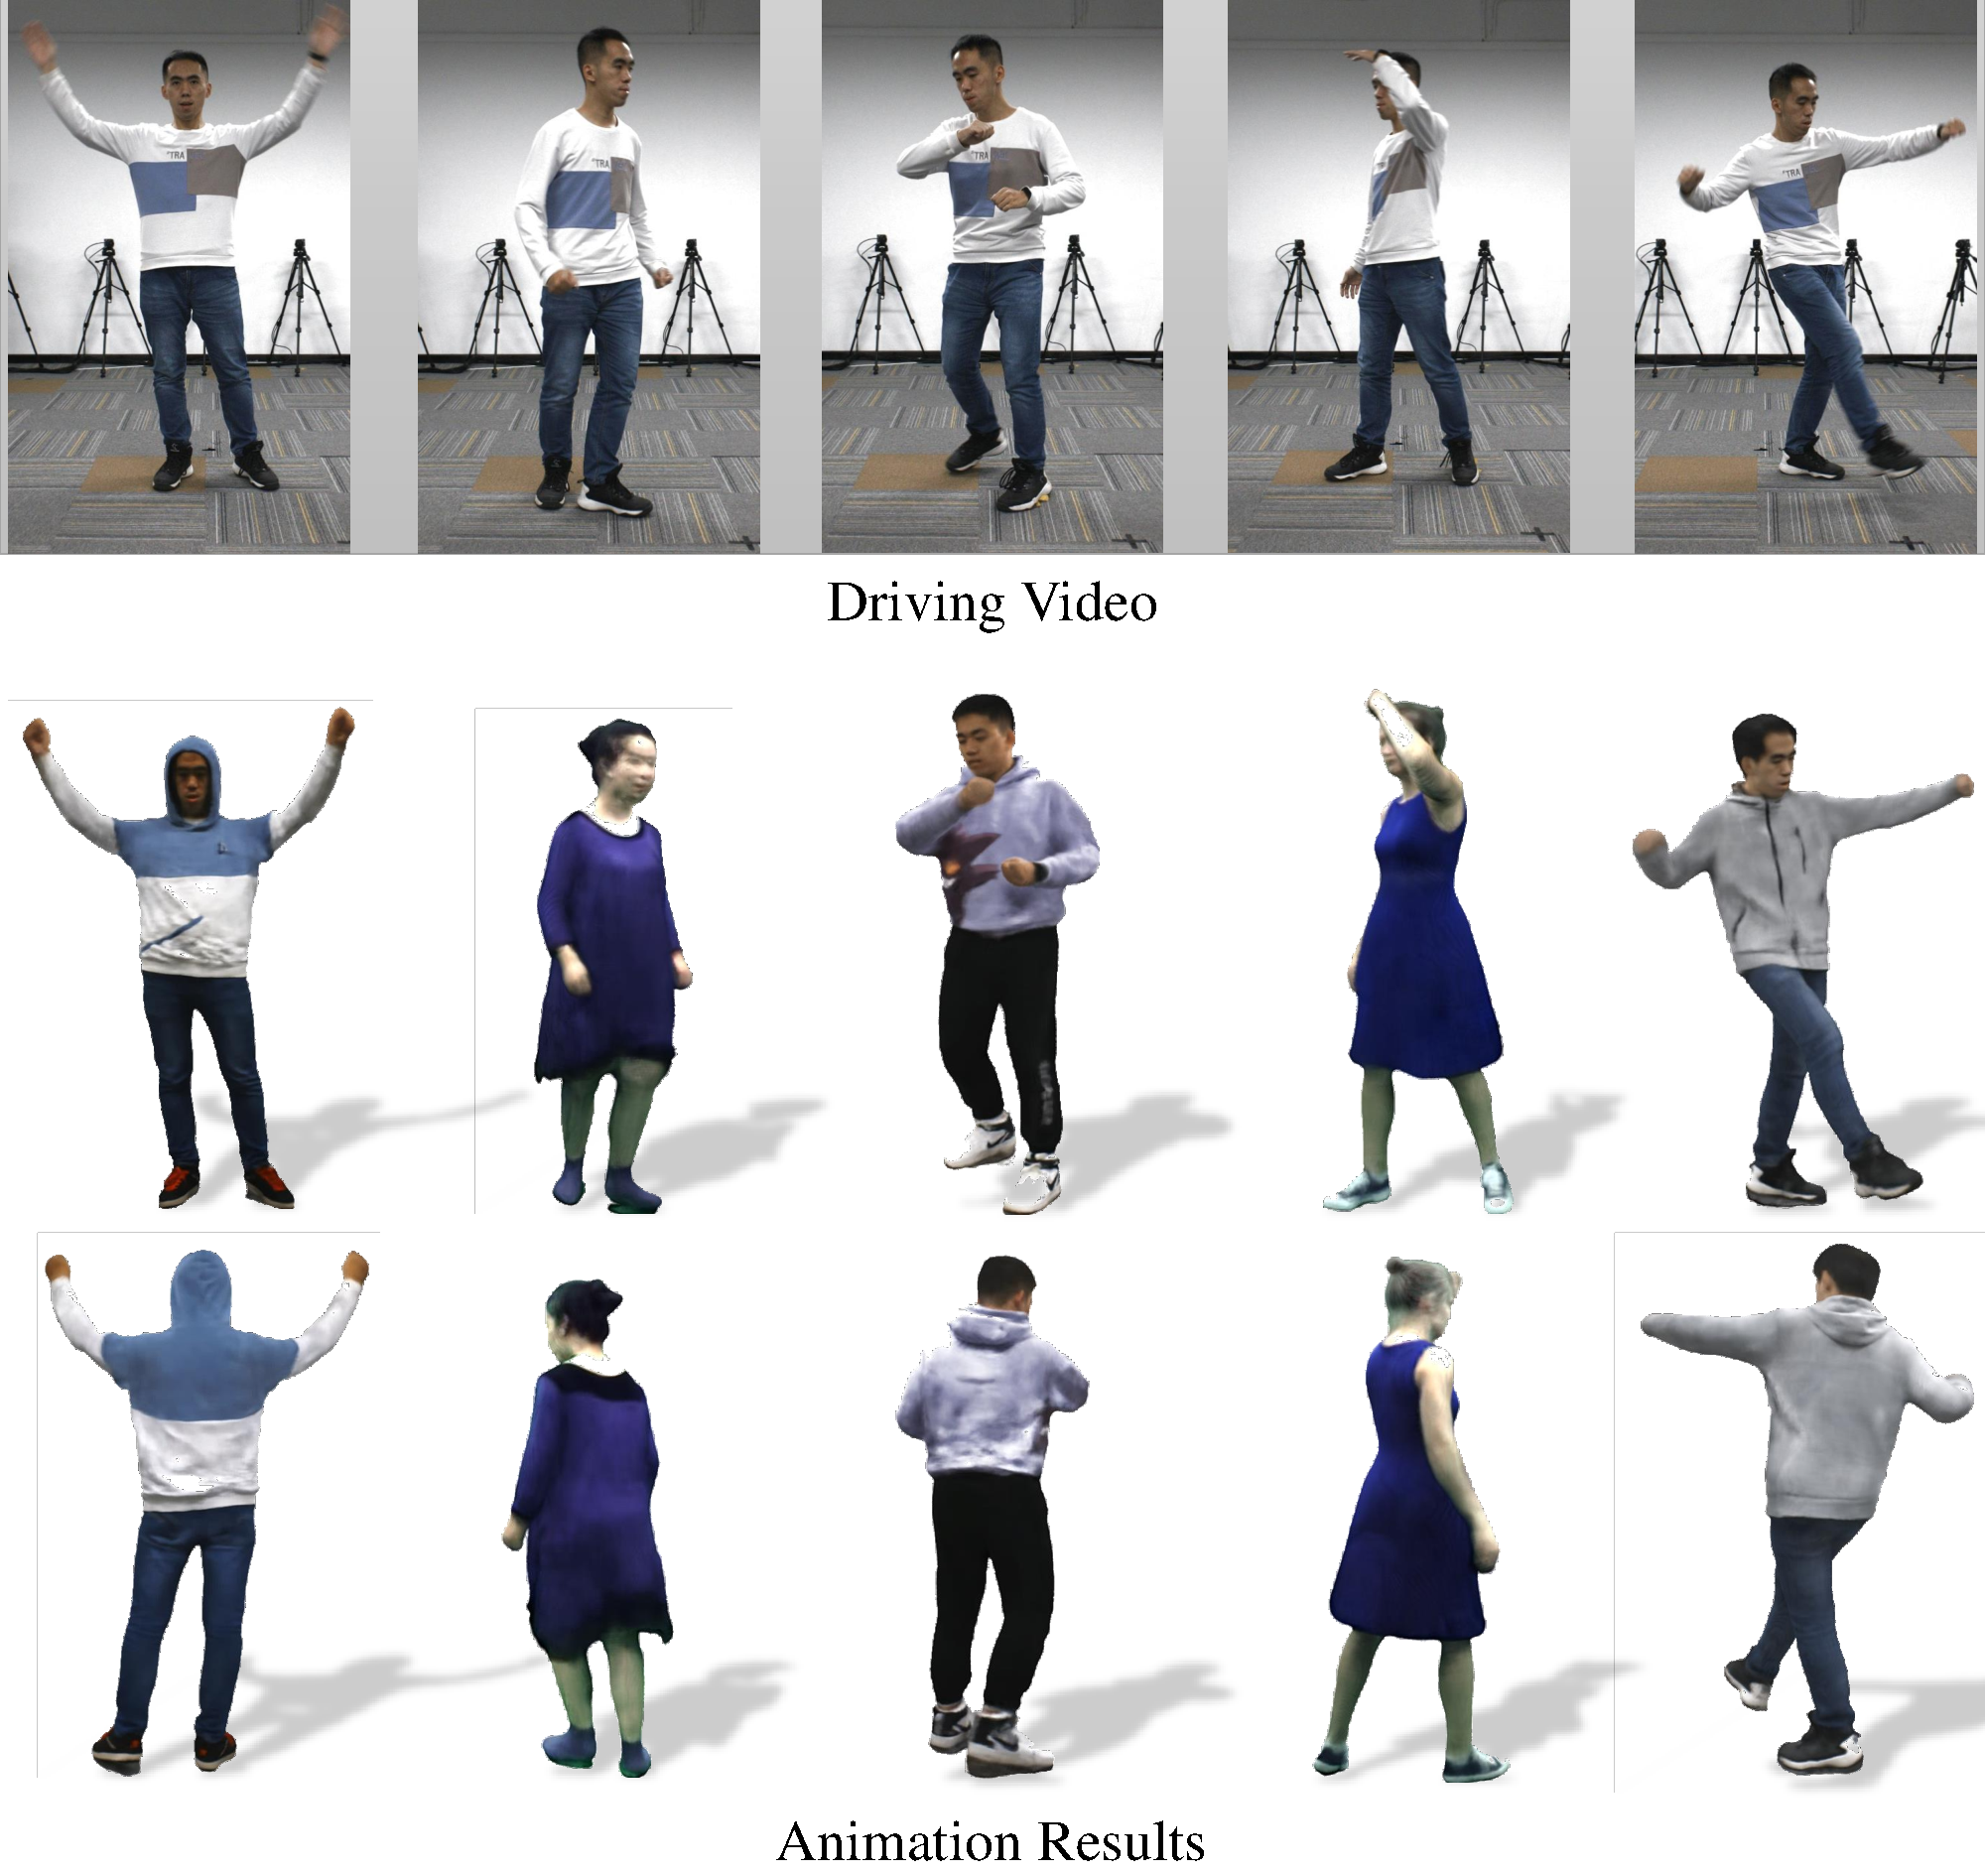
\includegraphics[width=\textwidth]{figures/teaser.pdf}
    \captionof{figure}{Overview of our method. \textbf{Left:} DiffMimic formulates motion mimicking as a straightforward state matching problem and uses analytical gradients to optimize it with off-the-shelf differentiable physics simulators. The formulation results in a simple optimization objective compared to heavy reward engineering in RL-based methods. \textbf{Middle:} DiffMimic is able to mimic highly dynamic skills, \eg, Side-Flip. \textbf{Right:} DiffMimic has a significantly better sample efficiency and time efficiency than state-of-the-art motion mimicking methods. Our approach usually achieves high-quality motion (pose error $<$ 0.15 meter) using less than $2\times10^7$ samples. }
    \label{fig:teaser}
\end{figure}
\section{Related works on debiasing}
\label{sec:related}

Addressing the issue of biased data and how it affects neural networks generalization has been the subject of numerous works.
Back in 2011, Torralba~and~Efros~\cite{torralba2011unbiased} showed that many of the most commonly used datasets are affected by biases. In their work, they evaluate the cross-dataset generalization capabilities based on different criteria, showing how data collection could be improved. 
With a similar goal, Tommasi~\emph{et~al.}~\cite{tommasi2017deeper} propose different benchmarks for cross-dataset analysis, aimed at verifying how different debiasing methods affect the final performances.
Data collection should be carried out with great care, in order not to include unwanted biases. Leveraging data already publicly available could be another way of tackling the issue. Gupta~\emph{et~al.}~\cite{gupta2018robot} explore the possibility of reducing biases by exploiting different data sources, in the practical context of sensors-collected data. They propose a strategy to minimize the effects of imperfect execution and calibration errors, showing improvements in the generalization capability of the final model. 
Khosla~\emph{et al.}~\cite{Khosla2012UndoingTD} employ max-margin learning (SVM) to explicitly model dataset bias for different vision datasets.
Another issue related to the unwanted learning of spurious correlations in the data has been highlighted by recent works. For example, Song~\emph{et~al.} \cite{song2017machine} and Barbano~\emph{et~al.}~\cite{barbano2021bridging} show how traditional training approaches allows information not relevant to the learning task to be stored inside the network. The experiments carried out in these works show how accurately some side information can be recovered, resulting in a potential lack of privacy.
Beutel~\emph{et~at.}~\cite{beutel2019putting} provide insights on algorithmic fairness in a production setting, and propose a metric named \emph{conditional equality}. They also propose a method, absolute correlation regularization, for optimizing this metric during training.
Another possibility of addressing these issues on a data level is to employ generative models, such as GANs~\cite{goodfellow2014generative}, to clean-up the dataset with the aim of providing fairness~\cite{xu2018fairgan, sattigeri2018fairness}.
Mandras~\emph{et~al.}~\cite{madras2018learning} also employ a GAN to obtain fair representations.

All of the above mentioned approaches generally deal directly at the data level, and provide useful insights for designing more effective debiasing techniques. 
In the related literature, we can most often find debiasing approaches based on ensembling methods, adversarial setups or regularization terms which aim at obtaining an \emph{unbiased} model using \emph{biased} data. We distinguish three different classes of approaches, in order of complexity: those which need full explicit supervision on the bias features (e.g. using bias labels), those which do not need explicit bias labels but leverage some prior knowledge of the bias features, those which no dot need neither supervision nor prior-knowledge.

\subsection{Supervised approaches}
Among the relevant related works, the most common debiasing techniques are supervised, meaning that they require explicit bias knowledge in form of labels. The most common approach is to use an additional bias-capturing model, with the task of specifically capturing bias features. This bias-capturing model is then leveraged, either in an adversarial or collaborative fashion, to enforce the selection of unbiased features on the main model. 
We can find the typical supervised adversarial approach in the work by Alvi~\emph{et~al.}: BlindEye~\cite{alvi2018turning}. They employ an explicit bias classifier, which is trained on the same representation space as the target classifier, using a min-max optimization approach. In this way, the shared encoder is forced to extract unbiased representations.
Similarly, Kim~\emph{et~al.}~\cite{Kim_2019_CVPR} propose Learning Not to Learn (LNL), which leverages adversarial learning and gradient inversion to reach the same goal.
Adversarial approaches can be found in many other works, for example in the work by Wang~\emph{et al.}~\cite{wang2019iccv}, where they show that biases can be learned even when using balanced datasets, and they adopt an adversarial approach to remove unwanted features from intermediate representations of a neural network. 
Also, Xie~\emph{et al.}~\cite{Xie2017ControllableIT} propose an adversarial framework for learning invariant representations with respect to some attribute in the data, similarly to~\cite{alvi2018turning}.
Moving away from adversarial approaches, Wang~\emph{et al.}~\cite{wang2020fair} perform a thorough review of the related literature, and propose a technique based on an ensemble of classifiers trained on a shared feature space.
A similar approach is followed by Clark~\emph{et~al.} with LearnedMixin~\cite{ClarkYZ19}. They train a biased model with explicit supervision on the bias labels, and then they build a robust model forcing its prediction to be made on different features.
Another possibility is represented by the application of adjusted loss functions or regularization terms.
For example, Sagawa~\emph{et~al.} propose Group-DRO~\cite{sagawa2019distributionally}, which aims at improving the model performance on the \emph{worst-group} in the training set, defined based on prior knowledge of the bias distribution.
EnD~\cite{tartaglione2021end}, which will be presented in detail in Section~\ref{sec:supervised-end}, also belongs to this class of approaches. 

\subsection{Prior-guided approaches}
In many real-world cases, explicit bias labels are not available. However, it might still be possible to make some assumptions or have some prior knowledge about the nature of the bias.
Bahng~\emph{et~al.}~\cite{bahng2019rebias} propose ReBias, an ensembling-based technique. Similarly to the work presented earlier, they build a bias-capturing model (an ensemble in this case). The prior knowledge about the bias is used in designing the bias-capturing architecture (e.g. by using a smaller receptive fields for texture and color biases). The optimization process, consists in solving a min-max problem with the aim of promoting independence between the biased representations and the unbiased ones.
A similar assumption for building the bias-capturing model is made by Cadene~\emph{et~al.} with RUBi~\cite{cadene2019rubi}. In this work, logits re-weighting is used to promote independence of the predictions on the bias features.
Borrowing from domain generalization techniques, another kind of approach aiming at learning robust representation is proposed by  Wang~\emph{et~al.} with HEX~\cite{wang2018learning}. They propose a differentiable neural-network-based gray-level co-occurrence matrix~\cite{haralick1973textural, lam1996glcm}, to extract biased textural information, which are then employed for learning invariant representations.
A different context is presented by Hendricks~\emph{et~al.}~\cite{hendricks2018women}. They propose an Equalizer model and a loss formulation which explicitly takes into account gender bias in image captioning models. In this work, the prior is given by annotation masks indicating which features in an image are appropriate for determining gender.
Related to this approach, another possibility is to constrain the model prediction to match some prior annotation of the input, as done in the work of Ross~\emph{et~al.}~\cite{Ross2017RightFT}, where gradients re-weighting is used to encourage the model to focus on the right input regions. Similarly, Selvajaru~\emph{et~al.}~\cite{Selvaraju_2019_ICCV} propose HINT, which optimizes the alignment between account manual visual annotation and gradient-based importance masks, such as Grad-CAM~\cite{selvaraju2017grad}.

\subsection{Unsupervised approaches}
Increasing in complexity, we consider as unsupervised approaches those methods which do not \emph{i)} require explicit bias information \emph{ii)} use prior knowledge to design specific architectures. 
In this setting, building a bias-capturing model is a more difficult task, as it should rely on more general assumptions. 
For example, Nam~\emph{et~al.} propose technique named Learning from Failure (LfF). They exploit the training dynamics: a bias-capturing model is trained with a focus on \emph{easier} samples, using the Generalized Cross-Entropy~\cite{zhang2018gce} (GCE) loss, which are assumed to be aligned with the bias, while a debiased network is trained emphasizing samples which the bias-capturing model struggles to learn. These assumptions they make are especially relevant for our work, as U-EnD also leverages the training dynamics for building the bias-capturing model. %
Similar assumptions are also made by Luo~\emph{et~al.}~\cite{luo2022pseudo} where GCE is also used for dealing with biases in a medical setting using Chest X-Ray images.
Ji~\emph{et al.}~\cite{ji2019invariant} propose an unsupervised clustering methods which is able to learn representations invariant to some unknown or ``distractor'' classes in the data, by employing over-clustering. Altough not strictly for debiasing purposes, another clustering-based technique is proposed by Gansbeke~\emph{et~al.}~\cite{van2020scan}: they employ a two-step approach for unsupervised learning of representations, where they mine the dataset to obtain pseudo-labels based on neighbours clusters. This approach is also closely related to our work.


\section{The EnD regularization}
\label{sec:supervised-end}



\begin{table}
   \center
    \caption{Overview on the notation used in this work.}
    \begin{tabular}{c l}%
        \toprule
        \textbf{Symbol} & \textbf{Meaning}\\
        \midrule
        $x_i$      & input ($i$-th sample in the dataset)\\
        $y_i$      & predicted class for the $i$-th sample \\
        $t_i$      & target class for the $i$-th sample \\
        $b_i$      & bias class for the $i$-th sample \\
        
        $Y$        & random variable associated to the predicted labels\\
        $T$        & random variable associated to the target labels\\
        $B$        & random variable associated to the bias labels\\
        $N_T$                     & cardinality of targets\\
        
        
        
        
        
        
      
        
        \bottomrule
    \end{tabular}
    \label{tab:notationover}
\end{table}

In this section we introduce the notation we adopt in this work, and provide a detailed explanation on how the EnD~\cite{tartaglione2021end} debiasing technique works in a supervised setting. Then, in Sec.~\ref{sec:unsupervised-end} we will move on to the unsupervised extension. 
The notation introduced in this work is summarized in Table~\ref{tab:notationover}\footnote{for the rest of this work, we conform to the standard notation proposed by Goodfellow~\emph{et~al.}~\cite{GoodBengCour16}, available at \url{https://github.com/goodfeli/dlbook\_notation}}.
Given a neural network \emph{encoder} $f(\cdot) \in R^N$ %
which extracts feature vectors of size $N$ and a \emph{classifier} $g(\cdot) \in R^{N_T}$ which provides the final prediction, we consider the neural network $(g~\circ~\gamma~\circ~f)(\cdot)$
where $\gamma : \mathbb{R}^N \rightarrow \mathbb{R}^N$ is a normalization function to obtain $z = \gamma(x) = x/\|x\|_2$.
The EnD regularization term $\mathcal{R}$ is applied jointly with the loss function $\mathcal{L}$ (e.g. cross-entropy), forcing $(\gamma \circ f)(\cdot)$ to filter out biased features from the extracted representation $z$. 
Hence, the overall objective function we aim to minimize is
\begin{equation}
    \label{eq:uprule}
    \mathcal{J} = \mathcal{L} + \mathcal{R},
\end{equation}
where $\mathcal{R}$ is the sum of the disentangling and entangling terms, weighted by two hyper-parameters $\alpha$ and $\beta$:
\begin{equation}
\label{eq:objective-func}
    \mathcal{R} = \alpha\mathcal{R}^{\perp} + \beta\mathcal{R}^{\parallel}
\end{equation}
Within a minibatch, let $i \in I \equiv \{1\dots M\}$ be the index of an arbitrary sample. We define $y_i$, $t_i$ and $b_i$ as the predicted, ground truth target and bias classes, respectively. 
The disentangling term $R^{\perp}$ is defined, for the $i$-th sample, as: 
\begin{equation}
	\mathcal{R}^{\perp}_{i} = \frac{1}{|B(i)|} \sum_{a \in B(i)} z_i \cdot z_a
\end{equation}
where $B(i) := \{j \in I \mid b_j = b_i  \} \setminus \{i\}$ is the set of all samples sharing the same bias class of $x_i$. 
The goal of this term is to suppress the common features among samples which have the same bias. %
The entangling term $R^{\parallel}$ is defined, for the $i$-th sample, as:
\begin{equation}
	\mathcal{R}^{\parallel}_{i} = - \frac{1}{|J(i)|}\sum_{j \in J(i)} z_i \cdot z_j
\end{equation}
where $J(i) := \{ j \in I \mid t_j = t_i \} \setminus B(i)$ is the set of all samples sharing the same target class of $x_i$ but with different biases. %
Complementarily to the disentangling term, the goal of this term is to encourage correlation among samples of the same class but with different bias, in order to introduce invariance with respect to the biased features.
So, for the $i$-th sample, the entire EnD regularization term $\mathcal{R}_i$ can be written as: 
\begin{equation}
\label{eq:end-full-new}
  \mathcal{R}_i =  \alpha\frac{1}{|B(i)|} \sum_{a \in B(i)} z_i \cdot z_a - \beta \frac{1}{|J(i)|}\sum_{j \in J(i)} z_i \cdot z_j \,. 
\end{equation}
The final $\mathcal{R}$ of Eq.~\ref{eq:objective-func}, is then just computed as the average over the minibatch: 

\begin{equation}
    \mathcal{R} = \frac{1}{M}\sum_i \mathcal{R}_i
\end{equation}
\begin{figure}
    \centering
    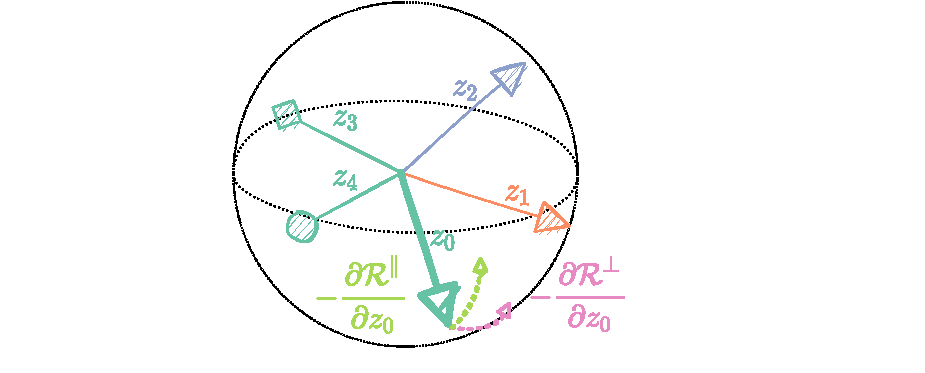
\includegraphics[width=0.6\columnwidth,trim={110 10 140 0},clip]{img/notation.pdf}
    \caption{Effect of the regularization term \eqref{eq:end-full-new} with respect to $z_0$. The features extracted from samples belonging to the same target class (same arrow's vertex) are entangled through the $R^\parallel$ term (in light green) while features for the same bias class (same color-in this case, with respect to $z_0$, dark green) are disentangled through the $R^\perp$ term (in pink).}
    \label{fig:notation}
\end{figure}
To visualize the effect of $\mathcal{R}$ as expressed in Eq.~\ref{eq:end-full-new}, consider a simple classification problem with three target classes and three different bias as illustrated in Fig.~\ref{fig:notation}. %
Training a model without explicitly addressing the presence of biases in the data, will most likely results in representations aligned by the bias attributes rather then the actual target class (Fig.~\ref{fig:notation}). 
The goal of $\mathcal{R}$ is to encourage the alignment of representations based on the correct features by \emph{i.)} disentangling representations of the same bias ($\mathcal{R}^\perp$) and \emph{ii.)} entangling representations of the same target in order to introduce invariance to the bias features ($\mathcal{R}^\parallel$).


\section{Unsupervised debiasing by subgroup discovery}
\label{sec:unsupervised-end}

\begin{figure*}
    \centering
    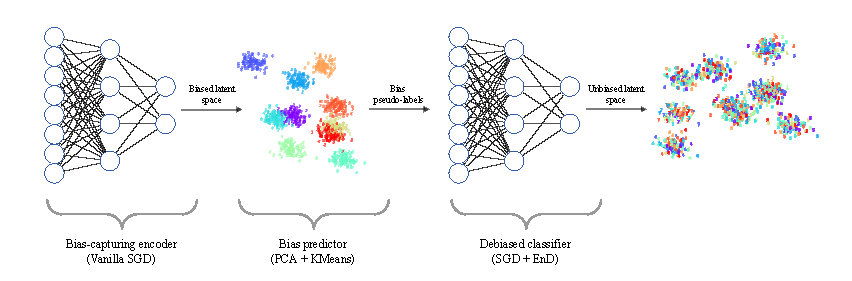
\includegraphics[width=\textwidth]{img/overview.pdf}
    \caption{Overview of our unsupervised debiasing approach: first we train a bias-capturing encoder, then we determine bias pseudo-labels with a bias predictor. Finally we employ the predicted labels for training a final debiased classifier. In this figure we use Biased MNIST~\cite{bahng2019rebias} as example, where the bias is given by a strong correlation between digit and color.}
    \label{fig:overview-unsupervised}
\end{figure*}

\begin{algorithm}
\DontPrintSemicolon
\SetKwBlock{stepA}{Train bias-capturing model}{end}
\SetKwBlock{stepB}{Train bias predictor}{end}
\SetKwBlock{stepC}{Train unbiased classifier}{end}
\KwIn{
    \begin{minipage}{.75\linewidth}
    Training and validation data $X^t = \{(x_i, y_i)\}$, $X^v = \{(\hat{x}_i, \hat{y}_i)\}$;
    Randomly initialized parameters $\theta_B = \{\theta_f, \theta_g\}$ and $\theta_D = \{\theta_f^D, \theta_g^D\}$ of the biased and unbiased classifiers.
    \end{minipage}
}
\BlankLine

\KwOut{Trained parameters $\theta_D$ of the unbiased classifier.}
\BlankLine

\stepA{
\par
Train the biased classifier using vanilla SGD: $\theta_B \leftarrow \text{SGD}(\theta_B, X^t)$\;
Compute the biased representations:
$Z^t = \{ f(x; \theta_f) \} \quad \forall x \in X^t$ and
$Z^v = \{ f(x; \theta_f) \}\quad\forall x \in X^v$\;
}

\stepB{
Compute the PCA projections $P^t, P^v$ of $Z^t,Z^v$\; 
Fit $k$ clusters on $P^v$ choosing the optimal $k$ based on silhoutte and compute the cluster centroids:
$\{\mu_1,...,\mu_k\} \leftarrow \text{KMeans}(P^v, k)$\;
Assign the pseudo-labels $\hat{b}_i \leftarrow \underset{b \leq k}{\arg\!\min}\,(P^t_i,\, \mu_b)$\; 
Update the training set $X^t \leftarrow \{(x_i, y_i, \hat{b}_i)\}$\;
}

\stepC{
Learn the parameters $\theta_D$ on $X^t$ searching the optimal $\alpha$ and $\beta$ on $X^v$:
$\theta_D \leftarrow \text{SGD}(\theta_D, X^t) + R(\theta^D_f, X^t, \alpha, \beta)$\;
}

\caption{General scheme of U-EnD}
\label{alg:overview}
\end{algorithm}

\noindent In this section we present our proposed unsupervised end-to-end debiasing approach, showing how an explicitly supervised technique such as EnD can be extended to the unsupervised case, where the bias labels are unavailable. 
We do this by showing how the bias information can be partially, and sometimes fully, recovered in a completely unsupervised manner. 
To achieve that, our proposed algorithm consists of three sequential steps, as illustrated in Fig.~\ref{fig:overview-unsupervised}. 
First, we train a bias-capturing classifier, employing standard optimization techniques (e.g. SGD or Adam);  
then, we recover bias-related information from the latent space of the biased classifier via clustering, in order to obtain a bias predictor, which we employ to categorize all of the training samples into different bias classes. Lastly, we apply the EnD debiasing technique using the predicted bias labels, in order to obtain a debiased classifier.
A general scheme of the entire pipeline can be found in Algorithm~\ref{alg:overview}. 
Throughout this work, we make the assumption that an \emph{unbiased} validation set is available: this is needed for searching the optimal EnD hyper-parameters.


\subsection{Training a bias-capturing model}
\label{sec:phase1}
The first step of our proposed algorithm is to train a bias-capturing model, which in our case is represented by a \emph{biased} encoder. To achieve this, we perform a vanilla training of a CNN classifier on the available training data. Here, we do not employ any technique aimed at dealing with the presence of biases in the data. The intuition of this approach is that 
if bias features are easier to learn than the desired target attributed, then the resulting model will also be biased. This has also been observed by other works. Following the definition proposed by Nam~\emph{et al.}~\cite{nam2020learning} we can identify two cases:

\begin{itemize}
    \item \emph{benign biases:} even if biases are present in the data, the model does not rely on bias related features as the target task is easier to learn;
    \item \emph{malignant biases:} biases are present in the data, and they are easier for the model to learn instead of the target task.
\end{itemize}

\noindent The latter case is the most relevant for our work, as malignant biases are those which result in a loss of performance when evaluating the model on an unbiased set.
Fig.~\ref{fig:overview-unsupervised} shows a visualization of the embeddings obtained with a biased encoder on the BiasedMNIST~\cite{bahng2019rebias} dataset, where the background color correlates very well with the target digit class, as shown in Fig.~\ref{fig:biased-mnist}.
It is clear how the different clusters emerging in the latent space correspond to the different background color, rather than to the actual digit.
This first step is summarized in Algorithm~\ref{alg:overview}, and we now provide a more formal description.
Let $\theta_B = \{\theta_f, \theta_g\}$ be the set of parameters of the bias-capturing model $p(x; \theta) = g(f(x; \theta_f); \theta_g)$ where $f$ and $g$ are the encoder and the classifier, respectively. The objective function we aim to minimize is the cross-entropy loss (CE):
\begin{equation}
    \label{eq:objective-fun-biased}
    \mathcal{L}_\text{CE}(p(x; \theta_B), q(x)) = -\sum_{t \in T} q(t|x) \log p(t|x;\theta_B)
\end{equation}
where $q(x)$ represents the ground truth class distribution. We say that there is a benign bias in the dataset, if we can identify some distribution $r(x)$, related to some other confounding factor in the data, such that there exists a set of parameters $\theta'$ which is a local minimizer of~\eqref{eq:objective-fun-biased} and
$\theta' = \arg\!\min_{\theta_B} \mathcal{L}_\text{CE}(p(x; \theta_B), r(x))$. 
If, additionally, $r(x)$ is also easier to approximate than $q(x)$, then the bias is malignant and by applying the optimization process we obtain a bias-capturing model.
Once the biased model is trained, we only consider the encoder $f(x; \theta_f)$, as we are interested in analyzing its latent space in order to retrieve bias-related information. 

\subsection{Fitting a bias predictor}
\label{sec:phase2}

The second step consists in obtaining a predictor which can identify the bias in the data. 
Based on the observations made in Section~\ref{sec:phase1}, we employ a clustering algorithm to categorize the extracted representations into different classes. As shown in Fig.~\ref{fig:overview-unsupervised}, the identified clusters correspond to the biases in the dataset.
In this work, we choose KMeans~\cite{lloyd1982least} as it is one of the most well-known clustering algorithms.
Given a set of representation $z = \{z_1, z_2,\dots, z_n\}$ extracted by $f(x; \theta_B)$ we aim to partition $z$ into $k$ sets $C = \{C_1, C_2, \dots, C_k\}$ in order to minimize the within-clusters sum of squares (WCSS), which can be interpreted as the distance of each sample from its corresponding cluster centroid, by finding: 
\begin{equation}
    \label{eq:kmeans-objective}
    \arg\!\min_C \sum_{i=1}^k \sum_{z \in C_i}|| z - \mu_i ||^2
\end{equation}
where $\mu_i$ is the centroid (average) of $C_i$.
Furthermore, once the clusters have been determined, 
it is very easy to use the determined centroids for classifying a new sample $\hat{z}$ based on its distance, simply by finding 
\begin{equation}
    \label{eq:kmeans-predict}
    \hat{b} = \arg\!\min_{i \leq k} ||\hat{z} - \mu_i||^2
\end{equation}
where $\hat{b}$ denotes the resulting pseudo-label. 
The KMeans algorithm requires a pre-specified number of clusters $k$: in this work, we automatically tune this parameter based on the
best silhouette score~\cite{rousseeuw87silhouetteCluster}, obtained by performing a grid search in the range $[2, 15]$. 
Considering that the representations obtained on the training set might be over-fitted, we choose to minimize \eqref{eq:kmeans-predict} on the validation set. Then, once the centroids of the clusters have been found, we use them for pseudo-labelling the training set.
Additionally, as KMeans is based on euclidean distance, which can yield poor results in highly dimensional spaces, we perform a PCA projection of the latent space before solving~\eqref{eq:kmeans-objective}~and~\eqref{eq:kmeans-predict}. For the same reasons as above, the PCA transformation matrix is also computed on the validation set.
We refer to the ensemble of the PCA+KMeans as \emph{bias predictor} model.
The cluster information is then used as bias pseudo-label, as explained in Section~\ref{sec:phase3}. 

\subsection{Training an unbiased classifier}
\label{sec:phase3}
The third and final step of our proposed framework consists in training an unbiased classifier using. For this purpose, we use the clusters discovered in the previous phase as pseudo-labels for the bias classes, as shown in Figure~\ref{fig:overview-unsupervised}. This allows us to employ the fully supervised EnD regularization term for debiasing. Here we follow the approach described in Section~\ref{sec:supervised-end}.
Denoting with $\theta_D = \{\theta_f^D, \theta_g^D\}$ the parameters of the encoder and the classifier of the debiased model $p'(x; \theta_D) = g(\gamma(f(x; \theta_f^D)); \theta_g^D)$.
The objective function that we aim to minimize in this phase is:
\begin{equation}
    \label{eq:objective-fun-unbiased}
    \mathcal{L}_\text{CE}(p'(x; \theta_D), q(x)) + R(\gamma(f(x; \theta_f^D)), q(x), b(x))
\end{equation}
where $b(x)$ is the distribution corresponding to the pseudo-labels computed in the clustering step of Section~\ref{sec:phase2}. The closer $b(x)$ is to the real distribution $r(x)$, the more minimizing~\eqref{eq:objective-fun-unbiased} will lead to minimizing $R$ with the respect to the unknown ground-truth bias labels.

\section{Analysis on controlled experiments}
\label{sec:analysis-mnist}

\begin{figure}
    \centering
    
\includegraphics[width=\columnwidth]{img/mnist.png}
    \caption{Biased MNIST by Bahng~\emph{et~al.} ~\cite{bahng2019rebias}. The bias is given by the correlation between digit and background color.}
    \label{fig:biased-mnist}
\end{figure}

In this section we provide more insights supporting the proposed solution. 
To aid in the explanation of the different steps of the algorithm, we employ the Biased-MNIST dataset~\cite{bahng2019rebias} as case study throughout this section. Biased-MNIST is built upon the original MNIST~\cite{lecun2010mnist} by injecting a color bias into the images background, as shown in Fig.~\ref{fig:biased-mnist}. 
A set of ten default colors associated with each image is determined beforehand. 
To assign a color to an image, the default color is chosen with a probability $\rho$, while any other color is chosen with a probability of $(1-\rho)$. 
More explicitly, given a label $i, 0 \leq i < N_T$ with $N_T=10$,
the probability distribution for each color is given by: 
\begin{equation}
    \begin{cases}
        P(B = i|T = i) = \rho \\
        P(B \neq i | T = i) = \frac{1}{N_T - 1} (1 - \rho)
    \end{cases}
    \label{eq:dist-b-given-t}
\end{equation}
where $B$ and $T$ are random variables associated to the bias and target class respectively.
The $\rho$ parameter allows us to determine the degree of correlation between background color (\emph{bias}) and digit class (\emph{target}). %
Hence, higher values of $\rho$ correspond to more difficult settings.
Following~\cite{bahng2019rebias}, we generate different biased training set, by selecting $\rho \in \{0.990, 0.995, 0.997, 0.999 \}$. In order to assess the generalization performance when training on a biased dataset, we construct an \emph{unbiased} test set generated with $\rho =\frac{1}{N_T} = 0.1$. Given the low correlation between color and digit class in the unbiased test set, models must learn to classify shapes instead of colors in order to reach a high accuracy. 

\begin{table}
    \centering
    \resizebox{\columnwidth}{!}{%
    \begin{tabular}{l c c c c}
        \toprule
        \multirow{2}{*}{Method} & \multicolumn{4}{c}{$\rho$ values}\\
                                & 0.999 & 0.997 & 0.995 & 0.990 \\ 
        \toprule
        Vanilla~\cite{bahng2019rebias} & 10.40\std{0.50} & 33.40\std{12.21} & 72.10\std{1.90} & \underline{89.10}\std{0.10} \\
        LearnedMixin~\cite{ClarkYZ19} & \underline{12.10}\std{0.80} & \underline{50.20}\std{4.50} & \underline{78.20}\std{0.70} & 88.30\std{0.70} \\
        EnD~\cite{tartaglione2021end} & \textbf{52.30}\std{2.39}    & \textbf{83.70}\std{1.03}  & \textbf{93.92}\std{0.35}  & \textbf{96.02}\std{0.08} \\
        \midrule
        HEX$^\dagger$~\cite{wang2018learning} & 10.80\std{0.40} & 16.60\std{0.80} & 19.70\std{1.90} & 24.70\std{1.60} \\
        RUBi$^\dagger$~\cite{cadene2019rubi} & 13.70\std{0.70} & 43.00\std{1.10} & \underline{90.40}\std{0.40} & \underline{93.60}\std{0.40}\\
        ReBias$^\dagger$~\cite{bahng2019rebias} & 22.70\std{0.40} & 64.20\std{0.80} & 76.00\std{0.60} & 88.10\std{0.60} \\
        U-EnD$^\dagger$ ($T$=80) & \underline{53.90}\std{4.03} & \underline{82.16}\std{0.63} & 74.39\std{0.43} & 88.05\std{0.16} \\
        U-EnD$^\dagger$ ($T$=10) & \textbf{55.29}\std{1.27} & \textbf{85.94}\std{0.33} & \textbf{92.92}\std{0.35} & \textbf{93.48}\std{0.06} \\
        \bottomrule
    \end{tabular}
    }
    \caption{Biased-MNIST accuracy on the unbiased test set. Techniques which can be used in an unsupervised way are denoted with $^\dagger$.}
    \label{table:mnist-results}
\end{table}

Experimental details are provided in the supplementary material. %
The results for Biased-MNIST are presented in Table~\ref{table:mnist-results}. We report the accuracy on the unbiased test set, obtained with the supervised EnD techique and the unsupervised extension. We also report reference results~\cite{bahng2019rebias} of other debiasing algorithms, both supervised and unsupervised. 
For U-EnD, we evaluate the results employing pseudo-labels computed at different training iterations ($T$) of the biased encoder: at an early stage after 10 epochs, and at a late stage at the end of training (80 epochs). In this section we focus on the late stage pseudo-labelling, while a detailed comparison between the two cases will be the subject of Section~\ref{sec:easy_first}.
Using the unsupervised method we are able to match the original performance of EnD with the ground-truth bias labels in most settings: this is true especially when the bias is stronger (higher $\rho$ values). This is because in these cases, the bias-capturing models will produce representations strongly biased towards the color, and the pseudo-labels obtained with the bias predictor model will be accurate. On the other hand, a slightly larger gap is observed when there is less correlation between target and bias features. 
This is the most difficult settings for the unsupervised clustering of the bias features: however, a significant improvement with respect to the baseline is always achieved. 
It may be argued that in such cases of weaker bias (or even absence of it), the representations extracted by the biased encoder will be more aligned with the target class rather the the bias features. In this case, the resulting pseudo-labels will be less representative of the actual bias, leading to the disentangling, instead, of the target labels. We identify two worst-case scenarios which might lead to inaccurate pseudo-labels: \emph{i.)} the training set is already unbiased, \emph{ii.)} the pseudo-labels we identify correspond to the target rather then to the bias labels. In this cases, applying a debiasing technique might lead to worse performance with respect to the baseline, however we are able to avoid this issue thanks to the hyper-parameters optimization policy that we employ. A more detailed analysis of the worst-case settings can be found in the supplementary material. %



\subsection{Easier patterns are preferred}
\label{sec:theoretical-model}

In this section we analyze how the bias affects the learning process, in order to provide a better understanding of the bias-capturing model.
By analyzing the training process at different values of $\rho$, we can identify when the color bias shifts from being benign to malignant. Fig.~\ref{fig:mnist-training} shows the training accuracy of vanilla models (the first step of our technique) trained with different values of $\rho$. Given that, in this case, the number of target classes and the number of different colors (bias classes) are the same, we are able to compute a bias \emph{pseudo-accuracy}
by finding the permutation of the predicted labels which maximizes the accuracy with respect to the ground truth bias labels: this gives value gives us an indication on how the final predictions of the model are aligned with the bias. 
From Fig.~\ref{fig:mnist-train} we observe that the target accuracy on the training set is, as expected, close to 100\%, while the bias accuracy is exactly the value of $\rho$, meaning that the models learned to recognize the digit.
This holds true also for the unbiased test set (Fig~\ref{fig:mnist-unbiased-test}), where the value $\rho=0.1$. However, if we focus on higher end of $\rho$ values (most difficult settings) as shown in Fig.~\ref{fig:mnist-unbiased-test-zoom}, we observe a rapid inversion in the trend: the target accuracy decreases, dropping to 10\% for $\rho=0.999$, while the bias accuracy becomes higher, close to 100\% towards the end of the $\rho$ range. In these settings, given the strong correlation between target and bias classes, it is clear that the bias has become easier for the model to learn, and thus malignant. These results can be viewed as further confirmation that neural networks tend to prefer and prioritize the learning of simpler patterns first, as noted by Nam~\emph{et~al.}~\cite{nam2020learning} and especially
Arpit~\emph{et~al.}~\cite{arpit2017memorization}: it is clear that, in order to be malignant, a bias must:

\begin{itemize}
    \item be an \emph{easier} pattern to learn that the target features;
    \item have a strong enough correlation with the target task.
\end{itemize}

\subsection{The effect of bias on learning}
\label{sec:bias-theoretical-model}
In order to provide a more in-depth understanding of the behaviour just described and to aid in the explanation of our debiasing technique, we propose a simple yet effective mathematical framework describing the impact of the bias on the learning process. 

Under the assumption that the target and biases classes are uniformly distributed across the dataset, we have:
\begin{align}
	H(T) &= -\sum_{i=1}^{N_T} P(t_i) \log_2 P(t_i) = \log N_T \nonumber \\
	H(B) &= -\sum_{j=1}^{N_T} P(b_j) \log_2 P(b_j) = \log N_T \label{eq:entropy_assumption}
\end{align}
where $T$ and $B$ are the random variables associated to the target and the bias class, respectively. Under the assumption of perfect learner, we must impose
   $H(Y|T) = 0$
(or in other words, the output $y_i$ of the model matches the ground truth value $t_i~\forall i$), and following the steps described in the supplementary material, %
we can write the \emph{normalized} mutual information
\begin{equation}
    \label{eq:MI_perfect}
	\widehat{I}_{perf}(B, Y) =  \log_{N_T}\left\{N_T\rho\left[\frac{1-\rho}{\rho(N_T-1)}\right]^{1-\rho}\right\}
\end{equation}
\begin{figure}
    \centering
    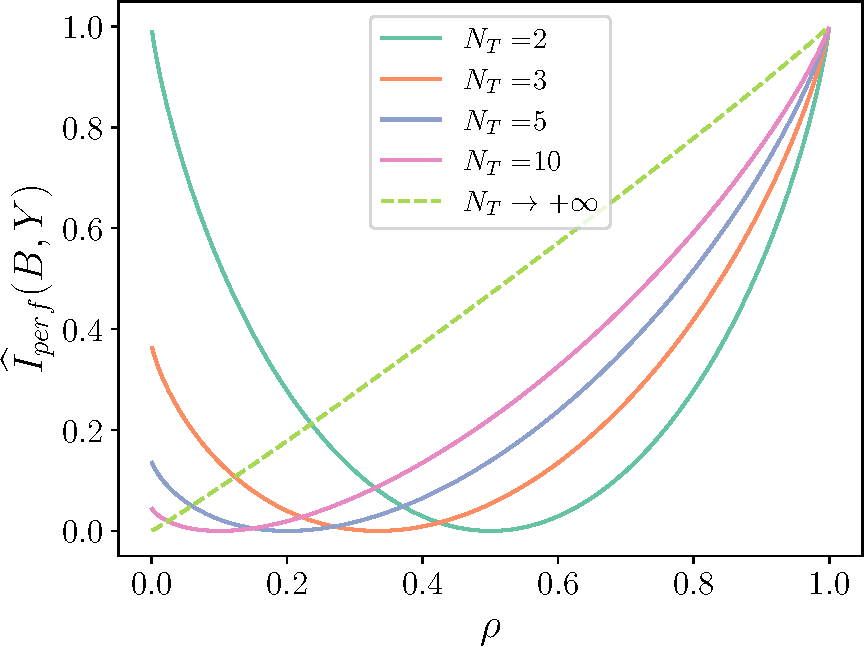
\includegraphics[width=\columnwidth]{img/MI_YZ.pdf}
    \caption{Normalized mutual information in case of perfect learner. As the number of classes $N_T$ increases, the curve smoothens. For low $N_T$ and low $\rho$ values, the anti-correlation phenomenon rises, and the mutual information increases.}
    \label{fig:MI_YZ}
\end{figure}
As it is possible to observe in Fig.~\ref{fig:MI_YZ}, a clear dependency between $\rho$ and \eqref{eq:MI_perfect} exists. In this case, the biased features and the target ones are in perfect overlap. Nonetheless, in the more general case the trained model is not a perfect learner, having $H(Y|T) \neq 0$.
The model, in this case, does not correctly classify the target for two reasons:
\begin{enumerate}
	\item It gets confused by the bias features, and it tends to learn to classify samples based on them. We model this tendency of learning biased features with $\phi$, which we call \emph{biasness}. The higher the biasness of is, the more the model relies on features which we desire to suppress, inducing bias in the model and for instance error in the model.
	\item Some extra error $\varepsilon$, non directly related to the bias features, which can be caused, for example, from stochastic unbiased effects, to underfit, or to other high-order dependencies between data. %
\end{enumerate}
We can write the discrete joint probability for $T, B, Y$, composed of the following terms.
\begin{itemize}
    \item When target, bias and prediction are aligned, the bias is aligned with the target class and correctly classified. Considering that we have not a prefect learner, we introduce the error term $\varepsilon$.
    \item When target and bias are align as well as bias and output, and the prediction is incorrect, it means that the model has not learned the correct feature and the bias is being contrasted.
    \item When target and bias are not aligned, but the prediction is correct and bias and output are aligned, it means that the model has learned the bias, introducing the error we target to minimize in this work.
    \item In all the other cases, the error of the model is due to higher-order dependencies, not directly related to the biasness $\phi$.
\end{itemize}
More formally, we can express the joint probability as:
\begin{align}
	P(T&,B,Y) = \frac{1}{N_T} \cdot \left[\delta_{tby} \rho (1 - \varepsilon) + \bar{\delta}_{ty}\delta_{tb}\delta_{by} \frac{(1-\phi)(1-\rho)}{N_T-1} \nonumber \right .\nonumber \\[1em]
	&+ \bar{\delta}_{tb}\delta_{ty}\delta_{by}\frac{\phi(1-\rho)}{N_T-1} + \delta_{tb}\bar{\delta}_{ty}\bar{\delta}_{by} \frac{\varepsilon \rho^2}{N_T-2+\rho} \nonumber \\[1em]
	&\left . + \bar{\delta}_{tb}\bar{\delta}_{ty}\bar{\delta}_{by} \frac{\varepsilon \rho (1-\rho)}{(N_T-1)(N_T-2+\rho)} \right]
    \label{eq:Pjointtotal}
\end{align}
where $\delta$ is the Kronecker delta function\footnote{for easiness of notation we suppress the index $i$: with $\delta_{tby}$ we implicitly intend that bias target and output are aligned to some $i$; hence $\delta_{ti}\delta_{bi}\delta_{yi}$}, $\bar{\delta}=1-\delta$ and $\phi,\varepsilon\in[0; 1]$.\footnote{not all the possible combinations are present in the joint probability \eqref{eq:Pjointtotal}: the missing combinations are  considered impossible, like having bias disaligned from the output but target aligned with the bias and with the output of the model (it would correspond to the case $\bar{\delta}_{by}\delta_{ty}\delta_{tb})$} We marginalize \eqref{eq:Pjointtotal} over $T$, obtaining
\begin{align}
	P(&B,Y) = \frac{1}{N_T} \cdot \left\{\delta_{by} [\rho (1 - \varepsilon) + \phi(1-\rho)] \right .\nonumber\\
	&\left .+ \bar{\delta}_{by}\left [\frac{(1-\phi)(1-\rho)}{N_T-1} + \frac{\rho\varepsilon}{N_T-2+\rho}\right ]\right\}
	\label{eq:joint_bz}
\end{align}
from which we compute the normalized mutual information
\begin{align}
    &\widehat{I}(B, Y) = \log_{N_T}\left[\rho (1 - \varepsilon) + \phi(1-\rho)\right]^{\rho (1 - \varepsilon)+ \phi(1-\rho)}\nonumber\\
    &+ \log_{N_T} \left [\frac{(1-\phi)(1-\rho)}{N_T-1} + \frac{\rho\varepsilon}{N_T-2+\rho}\right ]^{(1-\phi)(1-\rho) + \frac{(N_T-1)\rho\varepsilon}{N_T-2+\rho}}\nonumber\\
    &+ 1 + \rho\varepsilon \left(\frac{N_T-1}{N_T-2-\rho} -1 \right)\label{eq:MIcool}
\end{align}
\begin{figure}
    \centering
    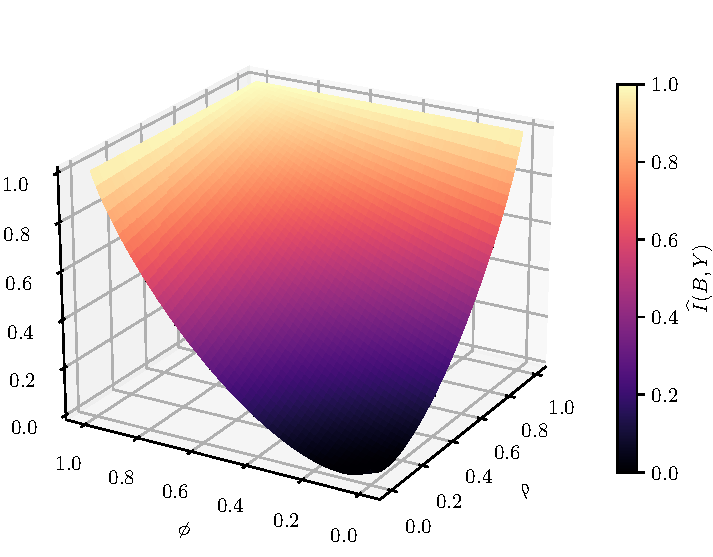
\includegraphics[width=1.0\columnwidth,trim={0 0 0 30},clip]{img/MI_YZ_full.pdf}
    \caption{Normalized mutual information between B and Y, in the case $\varepsilon=0$ and $N_T=10$. In light black, on top of the graph, level curves are drawn. In high $\rho$ regions, the mutual information is high regardless the bias tendency $\phi$ value, motivating the difficulty in learning the disentangling from biased features. A projection to a lower $\rho$ makes the problem of minimizing $\phi$ can drive the disentangling.}
    \label{fig:MI_YZ}
\end{figure}
The complete derivation can be found in the supplementary material %
and the plot for \eqref{eq:MIcool} in the case $\varepsilon=0$ is displayed in Figure~\ref{fig:MI_YZ}. 
Interestingly, we observe that for high values of $\rho$, the mutual information between the features
learned by the model and the bias is high, independently from the biasness $\phi$.
Typical learning scenarios, indeed, work in this region, where it is extremely challenging to optimize over $\phi$. On the contrary, with a lower $\rho$, the effect of $\phi$ appears evident. Towards this end, relying on a (relatively small) balanced validation set (hence, with low $\rho$) is extremely important in order to enhance the lowering of $\phi$. Directly optimizing over $\phi$ is in general not a duable strategy as the mutual information between B and Z in the typical training scenarios is very high; hence while bias removal can succeed, it will be extremely difficult to disentangle the biased features from the unbiased ones, without harming the performance.











\begin{figure*}
    \begin{subfigure}{0.33\textwidth}
        \centering
        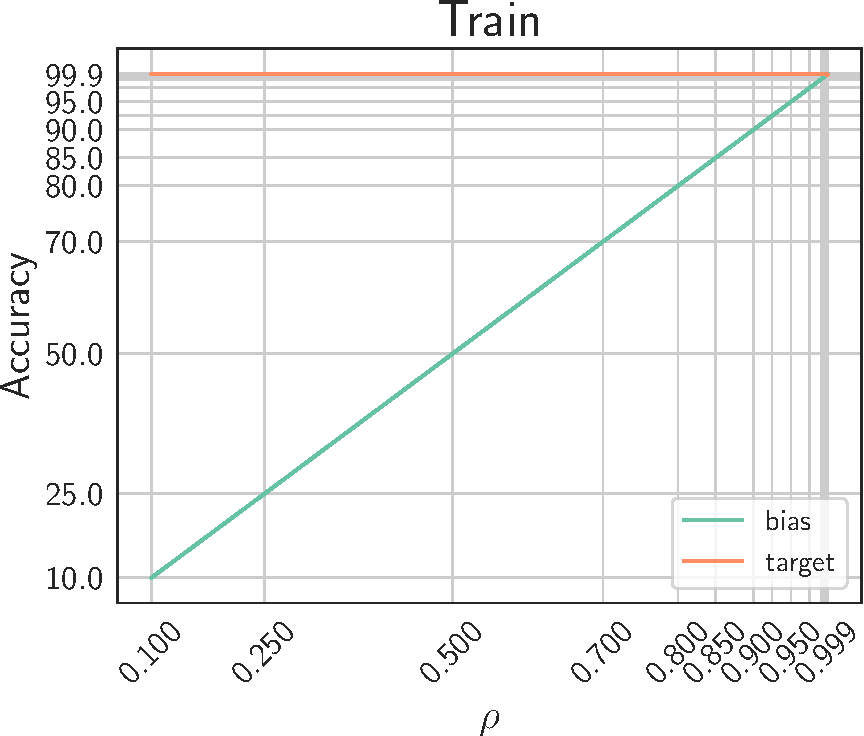
\includegraphics[width=\columnwidth]{img/mnist/train.pdf}
        \caption{~}
        \label{fig:mnist-train}
    \end{subfigure}
    \hfill
        \begin{subfigure}{0.33\textwidth}
        \centering
        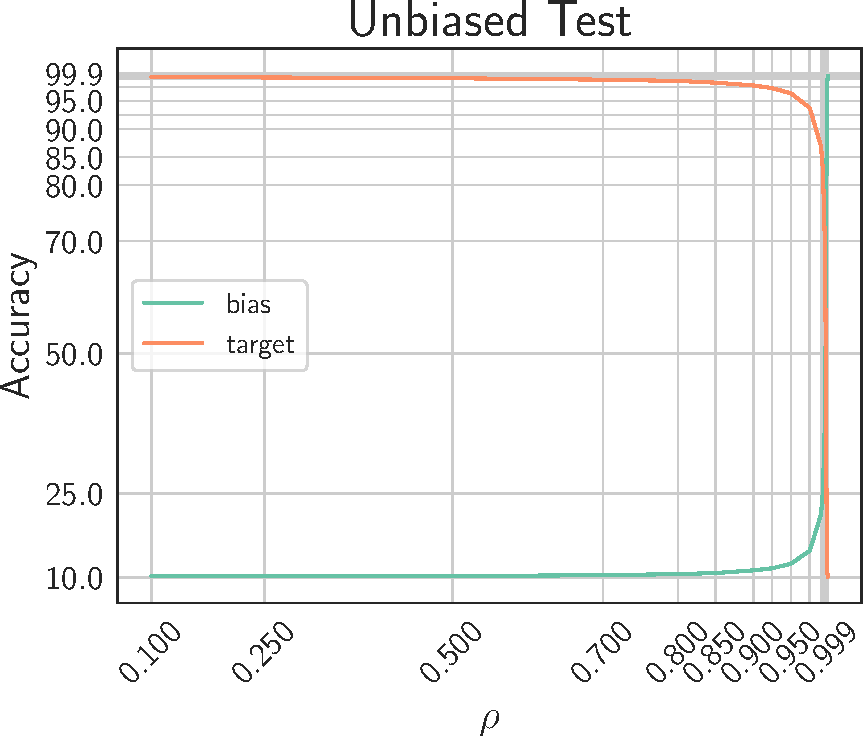
\includegraphics[width=\columnwidth]{img/mnist/unbiased_test.pdf}
        \caption{~}
        \label{fig:mnist-unbiased-test}
    \end{subfigure}
    \hfill
    \begin{subfigure}{0.33\textwidth}
        \centering
        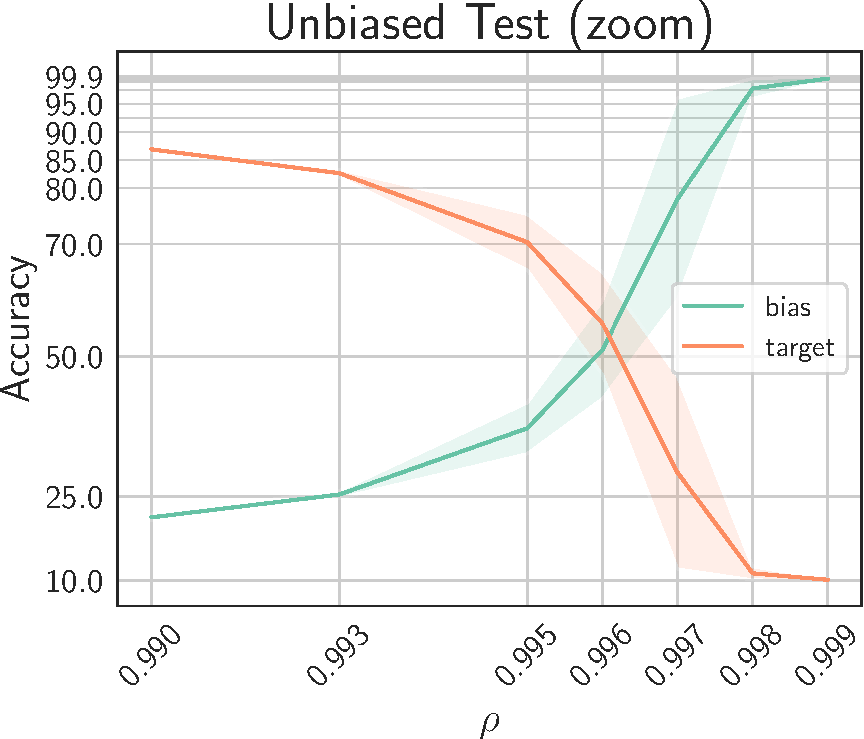
\includegraphics[width=\columnwidth]{img/mnist/unbiased_test_zoom.pdf}
        \caption{~}
        \label{fig:mnist-unbiased-test-zoom}
    \end{subfigure}
    
    \caption{Biased-MNIST accuracy on the training set (a), and on the unbiased test set (b) and (c). Results are reported in terms of mean and std across three different runs for every value of $\rho$. Given that the number of bias classes (colors) and target classes (digit) is the same, we can compute the bias accuracy by finding the permutation of predicted labels which maximizes the overlap with the ground truth bias labels.}
    \label{fig:mnist-training}
\end{figure*}

\subsection{Easier patterns are learned first}
\label{sec:easy_first}
Besides being easier to learn than the target task, we also find that biases tend to be learned in the first epochs. This is also evident when looking at the results in Table~\ref{table:mnist-results}, with $T=10$: using an early bias predictor results in more precise pseudo-labels, especially when $\rho$ is lower. In order to measure how biased the encoder is, we employ the theoretical model we presented in Eq.~\eqref{eq:joint_bz} to compute $\phi$ (the derivation can be found the supplementary material). %
In Fig.~\ref{fig:bias-tendency} we show the mean value of $\phi$ measured at different training iterations (we assume $\varepsilon=0$). As expected, the models tend to show stronger tendency towards bias when $\rho$ is higher. Interestingly, looking at the dynamics it is also clear that this behavior is exhibited predominantly in earlier epochs.
Under certain conditions, i.e. when the correlation between target and bias is not as strong, it is possible for the optimization process to escape the local minimum corresponding to a biased model. These findings are also confirmed by the related literature~\cite{nam2020learning, arpit2017memorization}. 

\begin{figure*}
    \centering
    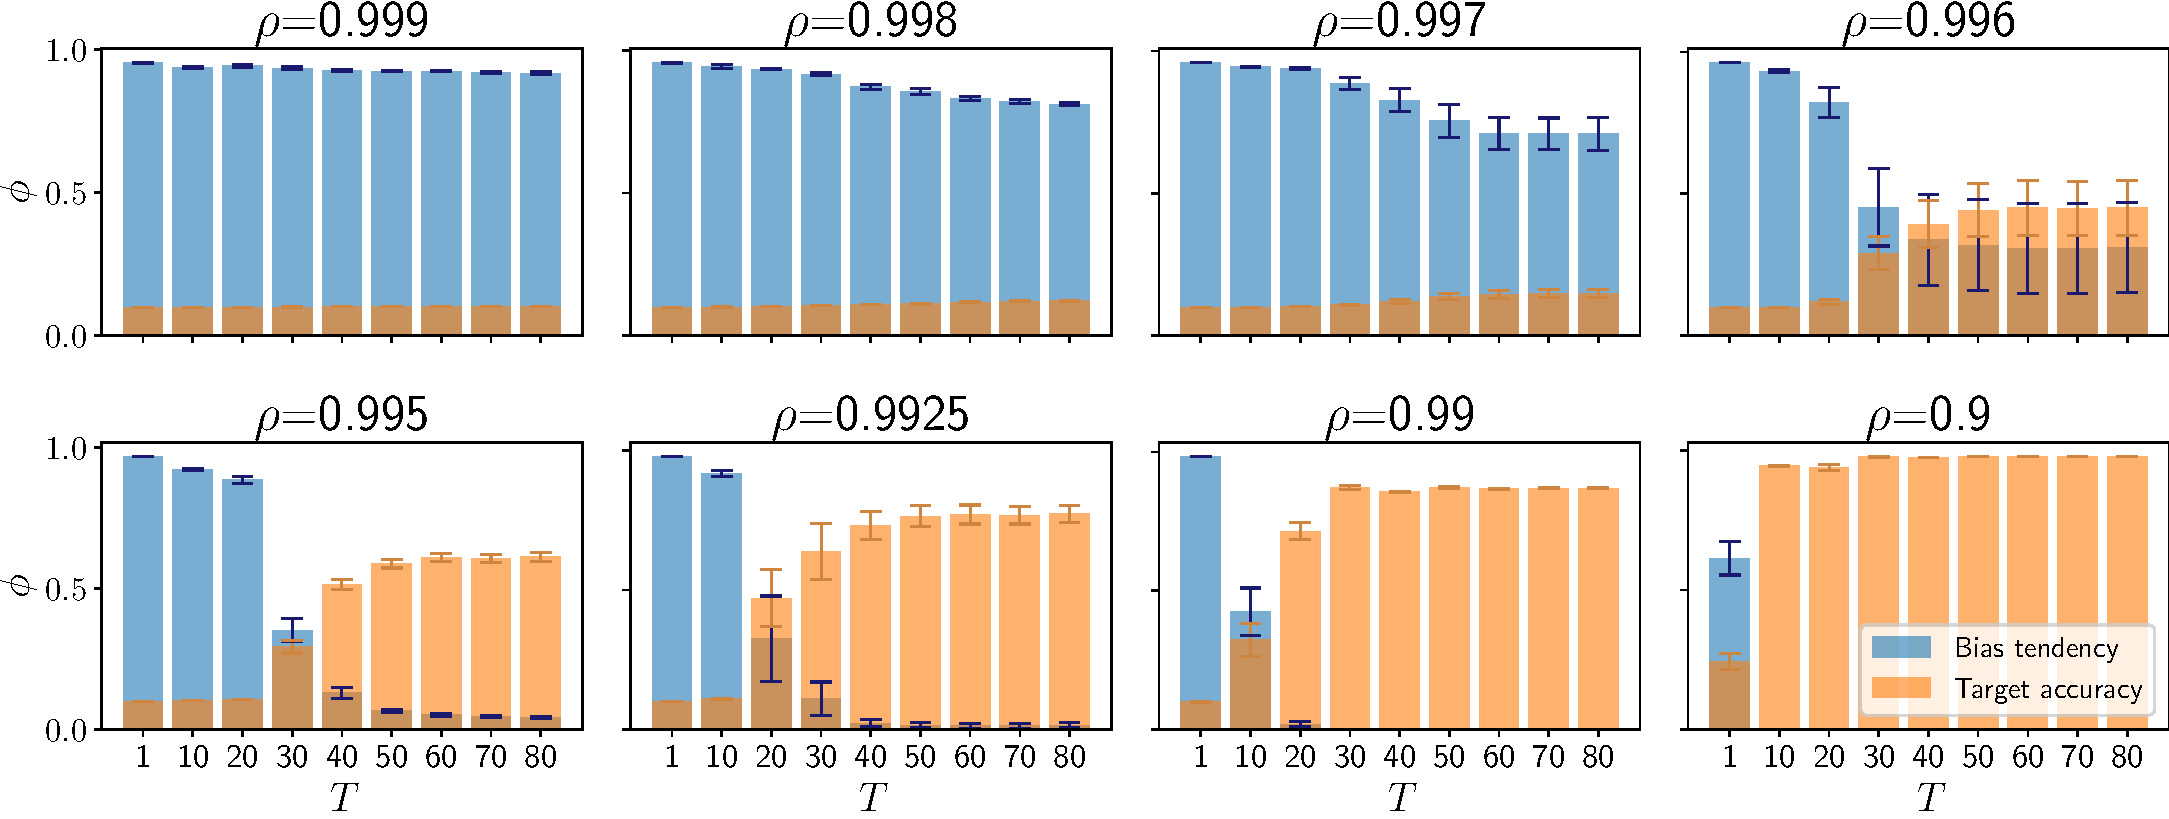
\includegraphics[width=\textwidth]{img/v.pdf}
    \caption{Biasness ($\phi$), or tendency towards learning bias features, in terms of mean and std computed across three independent runs for different values of $\rho$.}
    \label{fig:bias-tendency}
\end{figure*}



\section{Real world experiments}
\label{sec:experiments}


\begin{table}
    \centering
    \begin{tabular}{l@{\hspace{1\tabcolsep}} l@{\hspace{1\tabcolsep}} c c c}
        \toprule
        & Method & Unbiased & Bias-conflicting\\
        \midrule
        \multirow{6}{*}{\rotatebox{90}{Hair Color}}
        & Vanilla~\cite{nam2020learning} & 70.25\std{0.35} & 52.52\std{0.19} \\
        & Group DRO~\cite{sagawa2019distributionally} & \underline{85.43}\std{0.53} & \underline{83.40} \std{0.67}\\
        & EnD~\cite{tartaglione2021end} & \textbf{91.21}\std{0.22} & \textbf{87.45}\std{1.06}\\\addlinespace[1ex]
        \cline{2-4}\addlinespace[1ex]
        & LfF$^\dagger$~\cite{nam2020learning} & \underline{84.24}\std{0.37} & \textbf{81.24}\std{1.38} \\
        & U-EnD$^\dagger$ ($T$=50) & 83.97\std{2.90} & \underline{74.18}\std{6.07} \\
        & U-EnD$^\dagger$ ($T$=30) & \textbf{84.39}\std{2.38} & 72.53\std{4.47} \\
        \midrule
        \midrule
        \multirow{7}{*}{\rotatebox{90}{\small Heavy Makeup}}
        & Vanilla~\cite{nam2020learning} & 62.00\std{0.02} & 33.75\std{0.28} \\
        & Group DRO~\cite{sagawa2019distributionally} & \underline{64.88}\std{0.42} & \underline{50.24}\std{0.68} \\
        & EnD~\cite{tartaglione2021end} & \textbf{75.93}\std{1.31} & \textbf{53.70}\std{5.24}  \\\addlinespace[1ex]
        \cline{2-4}\addlinespace[1ex]
        & LfF$^\dagger$~\cite{nam2020learning} & 66.20\std{1.21} & \textbf{45.48}\std{4.33} \\
        & U-EnD$^\dagger$ ($T$=50) & \textbf{72.22}\std{0.00} & \underline{44.44}\std{0.00} \\
        & U-EnD$^\dagger$ ($T$=30) & \underline{67.59}\std{3.46} & 35.19\std{6.93} \\
        \bottomrule
    \end{tabular}
    \caption{\textbf{Performance on CelebA.} Techniques which can be used in an unsupervised way are denoted with $^\dagger$.}
    \label{table:celeba-results}
\end{table}


\begin{table}
    \centering
    \resizebox{\columnwidth}{!}{%
    \begin{tabular}{@{}l@{\hspace{0.8\tabcolsep}} l c c c c}
        \toprule
        &\multirow{2}{*}{Method}& \multicolumn{2}{c}{Trained on EB1} & \multicolumn{2}{c}{Trained on EB2} \\
        & & EB2 & Test & EB1 & Test \\
        \midrule
        \multirow{6}{*}{\rotatebox{90}{Learn Gender}}
        & Vanilla~\cite{Kim_2019_CVPR}                                & 59.86             & 84.42             & 57.84             & 69.75 \\
        & BlindEye~\cite{alvi2018turning}         & 63.74             & 85.56             & 57.33             & 69.90 \\
        & LNL~\cite{Kim_2019_CVPR}  & \underline{68.00} & 86.66 & 64.18 & 74.50 \\
        & EnD~\cite{tartaglione2021end}   & 65.49\std{0.81} & \underline{87.15}\std{0.31}  & \underline{69.40}\std{2.01}   & \underline{78.19}\std{1.18} \\
        & U-EnD$^\dagger$ ($T$=50) & \textbf{81.32}\std{2.17} & \textbf{90.98}\std{0.46} & \textbf{78.10}\std{0.70} & \textbf{83.03}\std{0.45} \\
        \midrule
        \multirow{6}{*}{\rotatebox{90}{Learn Age}} 
        &Vanilla~\cite{Kim_2019_CVPR}                                & 54.30 & 77.17 & 48.91 & 61.97 \\
        &BlindEye~\cite{alvi2018turning}        & 66.80 & 75.13 & {64.16} & 62.40 \\
        &LNL~\cite{Kim_2019_CVPR} & 65.27 & 77.43 & 62.18 & {63.04} \\
        & EnD~\cite{tartaglione2021end} & \underline{76.04}\std{0.25} & \underline{80.15}\std{0.96}  & \textbf{74.25}\std{2.26}  & \textbf{78.80}\std{1.48} \\  
        & U-EnD$^\dagger$ ($T$=50) & \textbf{80.41}\std{2.96} & \textbf{83.43}\std{2.49} & \underline{70.82}\std{1.04} & \underline{76.09}\std{0.91} \\
        \bottomrule
    \end{tabular}
    }
    \caption{\textbf{Performance on IMDB Face.} When gender is learned, age is the bias, and when age is learned the gender is the bias. Techniques which can be used in an unsupervised way are denoted with $^\dagger$.}
    \label{table:imdb-results}
\end{table}


In this section we present the experiments we performed on real-world datasets, where biases can be much harder to identify and overcome. In these experiments, we deal with different common kinds of biases in real datasets, 
specifically gender bias and age bias in facial images.
We use two very common datasets for facial recognition tasks, CelebA~\cite{liu2015faceattributes} and the IMDB face dataset~\cite{Rothe-IJCV-2018}. 

\subsection{Setup}
We use the common convolutional architecture ResNet-18 proposed by He~\emph{et~al.}~\cite{he2016deep}. The network is pre-trained on ImageNet~\cite{imagenetcvpr09}, except for the last fully connected layer. The same architecture is used both for training the biased encoder and the unbiased model. As in the previous experiments, the EnD regularization is applied on the encoder embeddings (average pooling layer). More experimental details are provided in the supplementary material
\footnote{Source code will be made pubicly available upon publication}.


\subsection{CelebA}
CelebA~\cite{liu2015faceattributes} is a widely known facial image dataset, comprising 202,599 images. It is built for face-recognition tasks, and provides 40 binary attributes for every image. 
Similarly to Nam~\emph{et al.}~\cite{nam2020learning}, we use attributes indicating the hair color and the presence of makeup as target attributes, while using the gender as bias. The reason is that there is a high correlation between these choices of attributes, with most of the woman in the dataset being blond or having heavy facial makeup.  We utilize the official train-validation split for training (162,770 images) and testing (19,867 images). As in~\cite{nam2020learning} we build two different testing datasets starting from the original one: an \emph{unbiased} set, in which we select the same number of samples for every possible pair of target and bias attributes, and a \emph{bias-conflicting}, where we only select samples where the values of target and bias attributes are different (e.g. men with blonde hair, women without makeup, and so on). This allows us to evaluate the model performance on the most difficult setting where the target is not aligned with the bias. Experimental details are provided in
the supplementary material. %

\subsubsection{Results} 
Denoting with $t$ and $b$ the target and bias attribute respectively, we computed the final accuracy as average accuracy across all the $(t, b)$ pairs, as in~\cite{nam2020learning}. We report the results in Table~\ref{table:celeba-results}. Results are reported for both the target attributes hair color and makeup. Techniques which can be used in an unsupervised manner are denoted with $^\dagger$. We report baseline results (vanilla) and we observe how vanilla models suffer significantly from the presence of the bias, scoring a quite low accuracy (especially since this is a binary task). This is evident on the bias-conflicting set, where the performance is close random-guess on hair color prediction, and even lower on the makeup detection. We report reference results~\cite{nam2020learning} of other debiasing algorithms, specifically Group~DRO~\cite{sagawa2019distributionally}, LfF~\cite{nam2020learning} and EnD~\cite{tartaglione2021end}. Focusing on supervised techniques (Group DRO and EnD) we observe a significant increase in performance, in both the tasks and test sets combinations. For the unsupervised methods, we report results of our U-EnD at different $T$ of the biased encoder, as done in Table~\ref{table:mnist-results}, and compare to LfF. We achieve better performance than the vanilla baseline in all settings, even though we still observe a gap with respect to the fully supervised techniques. The same observation can be made for LfF, which in general performs better on the harder cases in the bias-conflicting set, while U-EnD provides better performance in the more general case of the unbiased test set. 
The observed results are similar to the lower $\rho$ settings of BiasedMNIST: the amount of biased information is sufficient for it to be considered as a malignant bias, although it becomes slightly harder to perform pseudo-labeling in the biased encoder latent space. However, the assumptions we make in Sec.~\ref{sec:phase3} about the pseudo-labeling accuracy hold, resulting in better results with respect to the baseline models. 


\subsection{IMDB Face}
The IMDB Face dataset~\cite{Rothe-IJCV-2018} contains 460,723 face images annotated with age and gender information. This dataset is known to present noisy labels for age, thus Kim~\emph{et al.}~\cite{Kim_2019_CVPR} perform a cleaning step to filter out noisy labels from the data, by using a model trained on the Audience benchmark dataset~\cite{eidinger2014age}. Only the samples for which the original age value matches the predicted one are considered. As done in~\cite{Kim_2019_CVPR}, the filtered dataset is then split with a 80\%-20\% ratio between training and testing data. To construct a biased training set, the full training set subsequently  split into two \emph{extreme bias} (EB) sets: \emph{EB1}, which contains women only in the age range 0-29 and men with age 40+, and \emph{EB2} which contains man only in the age range 0-29 and women with age 40+. This way, a strong correlation between age and gender is obtained: when training age prediction, the bias is given by the gender, and when recognizing the gender, the bias is given by the age. 
Experimental details are provided in the supplementary material. %


\subsubsection{Results}
We report the results on the IMDB Face dataset in Table~\ref{table:imdb-results}, with regards to both gender and age prediction. Besides the test set, every model is also tested on the opposite EB set, to better evaluate the debiasing performance. As in the previous experiments, we use $^\dagger$ to denote the techniques which can be used in an unsupervised way. Focusing on the supervised techniques, we observe a significant improvement with respect to the baselines, especially with EnD and LNL, across the different combinations of test sets and task. Interestingly, in this case we are able to achieve even better results when employing the U-EnD approach, contrarily to the CelebA results. Especially for learning gender, we notice the the performance are noticeable higher than the best supervised results. This might be due to the noisy age labels in the dataset, and even if the described cleaning procedure is applied some labels could still be incorrect. With pseudo-labeling, on the other hand, we do not make use of the provided labels. This might be confirmed by the performances obtained when training for age prediction. As the gender label is of course far less noisy than the age, the performance gap between EnD and U-EnD is far less noticeable. We believe these results are very important, as they show that it is sometimes possible to achieve better results with unsupervised approaches.


\section{Conclusion}
\label{sec:conclusion}

In this work we proposed an unsupervised framework for learning unbiased representations from biased data. Our framework consists in three separate steps: \emph{i.)} training a bias-capturing model \emph{ii.)} training a bias predictor \emph{iii.)} training an unbiased model. 
We obtain the bias-capturing model by exploiting the tendency of optimization and neural networks to prefer simpler patterns over more complex ones. We show that when such patterns exist, and they represent spurious correlation with the target features, then the model will rely on these confouding factors. 
In Section~\ref{sec:phase1} we show that such case correspond to converging towards a local minimum for the target tasks, which however provides an optimal solver if we consider instead the task of predicting bias features. Furthermore, we the theoretical framework presented in Section~\ref{sec:bias-theoretical-model} we are able to empirically measure the biasness of the model, which can be a useful insights dealing with potentially biased data. We leverage this findings for adapting fully supervised debiasing techniques in unsupervised context, via a pseudo-labeling step on the biased latent space. Thanks to this approach, we are able to use state-of-the art debiasing algorithms such as EnD, which is a strong regularizer for driving the model towards the selection of unbiased features. With experiments on real-world data, we also show how sometimes it is even possible to achieve better results with an unsupervised approach, addressing the issue of noisy labels (both regarding target classes and bias classes) in datasets.
We believe that our approach could be of potentially great interest for other researchers in the area, and also for practical applications, as it can be easily adapted to different techniques for building bias-capturing models and for obtaining unbiased predictors.



\appendices
\section{Experimental details}
\label{appendix:experiments-details}

In this section we provide the detailed description of the setup for all the experiments presented.

\subsection{Biased-MNIST}
We use the network architecture proposed by Bahng~\emph{et~al.}~\cite{bahng2019rebias}, consisting of four convolutional layers with $7 \times 7$ kernels. The EnD regularization term is applied on the average pooling layer, before the fully connected classifier of the network. 
Following Bahng~\emph{et~al.}, we use the Adam optimizer with a learning rate of $0.001$, a weight decay of $10^{-4}$ and a batch size of 256. 
We train for 80 epochs. We do not use any data augmentation scheme. We use 30\% of the training set as validation set, and we colorize it using a $\rho$ value of 0.1.


\subsection{CelebA}

Following Nam~\emph{et~al.}~\cite{nam2020learning}, we use the Adam optimizer with a learning rate of $0.001$, a batch size of 256, and a weight decay of $10^{-4}$. We train for 50 epochs. Images are resized to $224\times224$ and augmented with random horizontal flip. To construct the validation set, we sample $N$ images from each pair $(t, b)$ of the training set, where $N$ is 20\% the size of the least populated group $(t, b)$. 
The EnD hyperparameters $\alpha$ and $\beta$ are searched using the Bayesian optimization~\cite{snoek2012practical} implementation provided by \emph{Weights and Biases}~\cite{wandb} on the validation set, in the interval $[0;50]$.
To provide a mean performance along with the standard deviation, we select the top 3 models based on the best validation accuracy obtained, and we report the average accuracy on the final test sets.

\subsection{IMDB}

We use the Adam optimizer with a learning rate of 0.001, a batch size of 256 and a weight decay of $10^{-4}$. We train for 50 epochs. As with CelebA, images are resized to $224\times224$ and randomly flipped at training time for augmentation. In this case, it is not possible to construct a validation set including samples from both EB1 and EB2, without altering the test set composition. Hence, we perform a 4-fold cross validation for every experiment. For example, when training on EB1, we use one fold of EB2 as validation set and the remaining three folds as EB2 test set. We repeat this process until each EB2 fold is used both as validation and as test set. The same process is repeated when training on EB2, by splitting EB1 in validation and test folds. When training for age prediction, we follow Kim~\emph{et ~al.}~\cite{Kim_2019_CVPR}, by binning the age values in the intervals 0-19, 20-24, 25-29, 30-34, 34-39, 40-44, 45-49, 50-54, 55-59, 60-64, 65-69, 70-100, proposed by Alvi~\emph{et~al.}~\cite{alvi2018turning}.
For every fold, the EnD hyperparameters $\alpha$ and $\beta$ are searched using the Bayesian optimization~\cite{snoek2012practical} implementation provided by \emph{Weights and Biases}~\cite{wandb} on the validation set, in the interval $[0;50]$.
To provide a mean performance along with the standard deviation, we select the top model for each fold, based on the best validation accuracy obtained. We report the accuracy obtained on the final test sets, as average accuracy among the different folds. 
\section{Additional empirical results}
\label{sec:extra-additional-results}
In this section we provide some additional results about our debiasing technique, mainly focusing on the worst-case scenarios described in Section~\ref{sec:analysis-mnist}. 


\begin{table}
    \centering
    \begin{tabular}{c c c}
         \toprule
         $\rho$ & Vanilla & EnD  \\
         \midrule
         0.1 & 99.21 & 99.24\std{0.05} \\
         \bottomrule 
    \end{tabular}
    \caption{Debiasing on an unbiased training set ($\rho=0.1$)}
    \label{table:mnist-unbiased-training}
\end{table}

\begin{table}
    \centering
    \begin{tabular}{c c c c}
        \toprule
        $\rho$ & Vanilla &  EnD (target) & EnD (random) \\
        \midrule
        0.995 & 72.10\std{1.90} & 72.25\std{0.56}  & 66.68\std{0.35} \\
        \bottomrule
    \end{tabular}
    \caption{Debiasing on incorrect bias labels. Target means that target labels are also used as bias label (i.e. $t_i = b_i$, worst case), random means that bias labels are assigned randomly.}
    \label{table:mnist-wrong-pseudo}
\end{table}

\subsection{Debiasing on an unbiased dataset}
\label{extra:debias-on-unbiased}

Here we show that the supervised EnD regularization does not deteriorate the final results if applied on a training set which is not biased. Table~\ref{table:mnist-unbiased-training} shows the results of training with EnD on Biased-MNIST with $\rho=0.1$.
In this setting, applying the regularization term is not harmful for obtaining good generalization: this is because in a supervised setting we still have access to the correct color labels, thus we do not perform disentanglement over any useful features for the network.
This is a trivial result, however with this demonstrated we can now focus on an unbiased training set in the unsupervised case.

\subsection{Debiasing with wrong pseudo-labels}
\label{extra:debias-on-wrong-bias}


\begin{figure}
    \centering
    \begin{subfigure}{0.8\columnwidth}
        \centering
        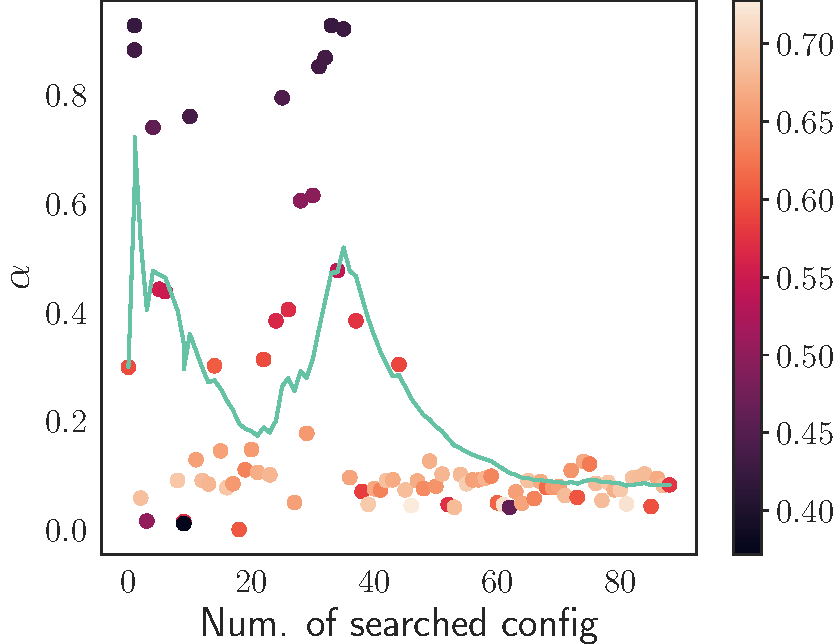
\includegraphics[width=1\columnwidth]{appendix/img/alpha_time.pdf}
        \caption{~}
        \label{fig:alpha-vs-time}
    \end{subfigure}\\[1em]
    \begin{subfigure}{0.8\columnwidth}
        \centering
        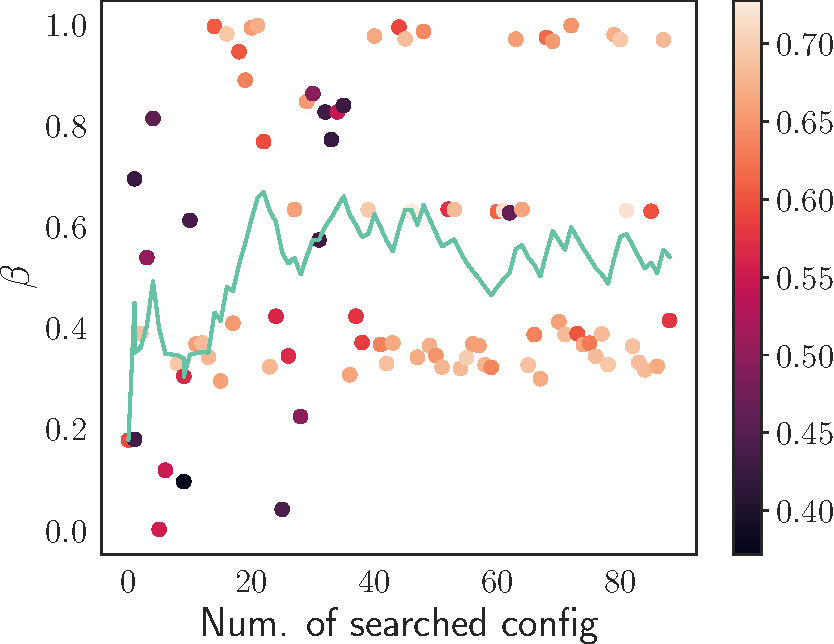
\includegraphics[width=1\columnwidth]{appendix/img/beta_time.pdf}
        \caption{~}
        \label{fig:beta-vs-time}
    \end{subfigure}

    \caption{{Evolution of (a) $\alpha$ and (b) $\beta$ versus the number of searched configs} during the hyperparameters optimization with incorrect pseudo-labels. We can observe how the optization process drives $\alpha$ towards 0, while $\beta$ does not seem to be revelant. The point color indicates the accuracy on the unbiased test set, while the line shows the trend as an exponetially weighted moving average computed with a smoothing factor of $0.1$.}
    \label{fig:alpha-beta-vs-time}
\end{figure}

We now assume that the pseudo-labels we compute are not representative of the true bias attributes. 
Using Biased-MNIST as case study, we identify that the worst-case scenario for the pseudo-labeling step corresponds to using a completely unbiased dataset (i.e. $\rho=0.1$) for training the biased encoder.
Taking into account the results shown in Section~\ref{extra:debias-on-unbiased}, performing the pseudo-labeling step in this setting this will most likely result in pseudo-labels corresponding to the actual target class rather then the background color.
We emulate this event by setting the bias label $b_i$ equal to the target label $t_i$ for every sample in the dataset, and then we the apply EnD algorithm. 
To test this worst-case with EnD, we choose $\rho=0.995$ as it provides a way for the final accuracy to both a decrease or increase with respect to a vanilla model. 
The results are reported in Table~\ref{table:mnist-wrong-pseudo}, and noted as \emph{target}. Even in this case, we are able to retain the baseline performances, altough we do not obtain any significant improvement. 
This is thanks to the hyperparameter optimization policy that we employ (recall that we assume an unbiased validation set - even if small - is available). 
Figure~\ref{fig:alpha-beta-vs-time} visualizes the evolution of the hyperparameters $\alpha$ and $\beta$ while searching for possibile configurations. 
In this setting, $\alpha$ represents the most dangerous term, as it enforces decorrelation among samples with the same class, conflicting with the cross-entropy term. 
However, the optimization process drivers $\alpha$ towards 0, making it effectively non-influent on the loss term. 
On the other hand, the entangling term $\beta$ does not bring any contribution to the learning process: it is, in fact, useless as there is full alignment between target and bias labels, hence $B(i)$ = \O. 
A possible scenario in which $\beta$ would not have null influence, is if we do not impose $t_i = b_i$. 
We explore the extreme setting by assigning a random value to $b_i$ for every sample $i$. The results are reported as \emph{random} in Table~\ref{table:mnist-wrong-pseudo}. In this case it is possible to observe a drop in performance with respect to the baseline. However, we argue that random pseudo-labels would be the result of poor representations due to possibly underfitting models or lack of sufficient training data - which, in a practical setting, would be a more pressing issue. 
\section{Complete derivations for Section~\ref{sec:bias-theoretical-model}}

In this section we present the full derivations of the theoretical results.

\subsection{Derivation of \eqref{eq:MI_perfect}}
\label{appendix:MI_perfect}
Let \eqref{eq:entropy_assumption}, we can write the conditional entropy
\begin{align}
    H_{perf}&(B|Y) = -\sum_{i=1}^{N_T} P(y_i) \sum_{j=1}^{N_T} P(b_j | y_i) \log_{2} \left [P(b_j | y_i) \right ]\nonumber\\
    =& -\frac{1}{N_T} \sum_{i=1}^{N_T} \sum_{j=1}^{N_T} P(b_j | y_i) \log_{2} [P(b_j | y_i)]\nonumber\\
    =& -\frac{1}{N_T}  \sum_{i=1}^{N_T} \sum_{j=1}^{N_T} \left\{ [\rho \log_{2}(\rho)] \delta_{ij} +\right .\nonumber\\
    &\left . +\left[\frac{1-\rho}{N_T-1} \log_{2}\left(\frac{1-\rho}{N_T-1}\right)\right]\overline{\delta}_{ij} \right\}\nonumber\\
    =& -\frac{1}{N_T} \left\{ N_T\cdot [\rho \log_{2}(\rho)] +\right .\nonumber\\
    &\left . +(N_T^2 - N_T)\cdot\left[\frac{1-\rho}{N_T-1}\cdot \log_{2}\left(\frac{1-\rho}{N_T - 1}\right)\right]\right\}\nonumber\\
    =& - \rho \cdot \log_{2}(\rho) +\nonumber\\
    & - \left\{(1-\rho)\cdot [\log_{2}(1-\rho) - \log_{2}(N_T-1)]\right\}\nonumber\\
    =& - \rho \cdot \log_{2}(\rho) - \log_{2}(1-\rho) +\log_{2}(N_T-1) +\nonumber\\
    & + \rho \cdot \log_{2}(1-\rho) - \rho \cdot\log_{2}(N_T-1)\nonumber\\
    =& \rho \cdot \log_{2}\left[\frac{1-\rho}{(N_T-1) \cdot\rho}\right] + \log_{2}\left[\frac{N_T-1}{1-\rho}\right]\nonumber\\
    =& \log_{2}\left[\frac{1-\rho}{N_T-1}\right]^{\rho-1} + \rho \log_2 \rho\nonumber\\
    =& -\log_{2}\left[\frac{1-\rho}{N_T-1}\right]^{1-\rho} + \log_2 \rho\cdot \rho^{\rho-1}\nonumber\\
    =& -\log_{2}\rho\left[\frac{1-\rho}{\rho(N_T-1)}\right]^{1-\rho}
\end{align}

Once we have the conditional entropy, we can compute the mutual information

\begin{align}
    I_{perf}(B, Y) &= H(B) - H_{perf}(B|Y)\nonumber\\
    &= \log_2 N_T +\log_{2}\rho\left[\frac{1-\rho}{\rho(N_T-1)}\right]^{1-\rho}
\end{align}

from which, exploiting \eqref{eq:entropy_assumption}, we can obtained the normalized mutual information
\begin{align}
    \hat{I}_{perf}(B,Y) =& \frac{2\cdot I_{perf}(B, Y)}{H(B) + H(Y)}\nonumber\\
    =&\frac{2\cdot\left\{ \log_2 N_T +\log_{2}\rho\left[\frac{1-\rho}{\rho(N_T-1)}\right]^{1-\rho}\right\}}{2\cdot \log_2 N_T}\nonumber\\
    =& 1 + \log_{N_T}\left\{\rho\left[\frac{1-\rho}{\rho(N_T-1)}\right]^{1-\rho}\right\}\nonumber\\
    =& \log_{N_T}\left\{N_T\rho\left[\frac{1-\rho}{\rho(N_T-1)}\right]^{1-\rho}\right\}\nonumber
\end{align}

\subsection{Derivation of \eqref{eq:MIcool}}
\label{appendix:MI}
Let the marginal as in \eqref{eq:joint_bz}. Following the definition of mutual information, we can write
\begin{align}
    I&(B,Y) = \sum_{i,j} P(b_j,y_i) \log_2\frac{P(b_j,y_i)}{P(b_j)P(y_i)}\nonumber\\
    =&\frac{1}{N_T} \left\{ N_T \cdot\left[\rho (1 - \varepsilon) + \phi(1-\rho) \right] \cdot \right.\nonumber \\
    &\cdot \log_2 (N_T \cdot(\rho (1 - \varepsilon) + \phi(1-\rho))) +\nonumber \\
    &+ (N_T^2 - N_T) \cdot \left [\frac{(1-\phi)(1-\rho)}{N_T-1} + \frac{\rho\varepsilon}{N_T-2+\rho}\right ]\cdot\nonumber\\
    &\left .\cdot \log_2 \left[ N_T \cdot \left(\frac{(1-\phi)(1-\rho)}{N_T-1} + \frac{\rho\varepsilon}{N_T-2+\rho}\right)\right ] \right\}\nonumber\\
    =&\left[\rho (1 - \varepsilon) + \phi(1-\rho) \right] \cdot \nonumber\\
    &\cdot \left[\log_2 N_T + \log_2(\rho (1 - \varepsilon) + \phi(1-\rho)\right] + \nonumber\\
    &+ \left [(1-\phi)(1-\rho) + \frac{(N_T - 1)\rho\varepsilon}{N_T-2+\rho}\right ]\cdot\nonumber\\
    &\cdot \left[ \log_2 N_T + \log_2 \left(\frac{(1-\phi)(1-\rho)}{N_T-1} + \frac{\rho\varepsilon}{N_T-2+\rho}\right)\right ]\nonumber\\
    =&\log_2\left[\rho (1 - \varepsilon) + \phi(1-\rho)\right]^{\rho (1 - \varepsilon) + \phi(1-\rho)} +\nonumber\\
    &+ \log_2 \left(\frac{(1-\phi)(1-\rho)}{N_T-1} + \frac{\rho\varepsilon}{N_T-2+\rho}\right)^{(1-\phi)(1-\rho) + \frac{(N_T - 1)\rho\varepsilon}{N_T-2+\rho}}+\nonumber\\
    &+\log_2 N_T \left[\rho (1 - \varepsilon) + \phi(1-\rho) + (1-\phi)(1-\rho) + \frac{(N_T - 1)\rho\varepsilon}{N_T-2+\rho}\right ]\nonumber\\
    =&\log_2\left[\rho (1 - \varepsilon) + \phi(1-\rho)\right]^{\rho (1 - \varepsilon) + \phi(1-\rho)} + \nonumber\\
    &+ \log_2 \left(\frac{(1-\phi)(1-\rho)}{N_T-1} + \frac{\rho\varepsilon}{N_T-2+\rho}\right)^{(1-\phi)(1-\rho) + \frac{(N_T - 1)\rho\varepsilon}{N_T-2+\rho}}+\nonumber\\
    &+\log_2 N_T \left[1-\rho\varepsilon + \frac{(N_T - 1)\rho\varepsilon}{N_T-2+\rho}\right ]\label{eq:IBZA}\\
\end{align}
Similarly to how been done in Sec.\ref{appendix:MI_perfect}, we can obtain the normalized mutual information
\begin{align}
    \hat{I}&(B,Y) = \frac{2\cdot I(B, Y)}{H(B) + H(Y)} = \frac{I(B, Y)}{\log_2 N_T}\nonumber\\
    =& \log_{N_T}\left[\rho (1 - \varepsilon) + \phi(1-\rho)\right]^{\rho (1 - \varepsilon)+ \phi(1-\rho)}\nonumber\\
    &+ \log_{N_T} \left [\frac{(1-\phi)(1-\rho)}{N_T-1} + \frac{\rho\varepsilon}{N_T-2+\rho}\right ]^{(1-\phi)(1-\rho) + \frac{(N_T-1)\rho\varepsilon}{N_T-2+\rho}}\nonumber\\
    &+ 1 - \rho\varepsilon + \frac{(N_T-1)\rho\varepsilon}{N_T-2-\rho}\nonumber
\end{align}
which in this case results in a simple change of base for the logarithms in \eqref{eq:IBZA}.

\subsection{Derivation of biasness}
\label{appendix:v-derivation}
Using the theoretical model presented in Section~\ref{sec:theoretical-model}, we can compute $\phi$ by rewriting of Eq.~\ref{eq:joint_bz} in order to derive it. First, for easier readibility, we explicitly enumerate the cases given by the kronecker deltas of Eq.~\ref{eq:joint_bz}:
\begin{equation}
    P(b, y) = 
\begin{cases}
    \frac{1}{N_T} \left[\rho (1 - \varepsilon) + \phi(1-\rho) \right] \quad \text{if } b=y \\[2ex]
	\frac{1}{N_T}\left [\frac{(1-\phi)(1-\rho)}{N_T-1} + \frac{\rho\varepsilon}{N_T-2+\rho} \right]  \quad \text{if } b \neq y
\end{cases}
\end{equation}
From this, we can rewrite each case in order to obtain the bias tendency $\phi_{b,y}$ for each $b$ and $y$:
\begin{equation}
    \phi_{b,y} = 
\begin{cases}
     P(b, y)\frac{N_T}{1 - \rho} - \frac{\rho(1-\varepsilon)}{1 - \rho} \quad \text{if } b = y \\[2ex]
     1 - P(b,y)\frac{N_T^2-N_T}{1-\rho} + \varepsilon\frac{\rho(N_T-1)}{(1-\rho)(N_T-2-\rho)} \quad \text{if } b \neq y
\end{cases}
\end{equation}
Note that, by doing so, we are actually computing multiple $\phi$ values, as a function of $b$ and $y$, while in Eq.~\ref{eq:joint_bz} we assume the values to be constant (i.e. the bias tendency is the same independently from the value of $b$ and $y$ considered). 
In our experiments, to account for the assumptions we make ($\varepsilon = 0$) and for measurements errors due to the stochastic nature of the training, we clip the measured joint probability between $[\frac{\rho}{N_T}; \frac{1}{N_T}]$ for the diagonal values ($b=y$), and between $[0; \frac{1-\rho}{N_T(N_T-1)}]$ for the off-diagonal values ($b \neq y$). This ensures that the computed $\phi_{b,y}$ lies between the valid range $[0; 1]$.
Finally, we can compute the global $\phi$ by averaging all the $\phi_{b,y}$:
\begin{equation}
\phi = \frac{1}{N_B N_T}\sum_{b,y} \phi_{b,y}
\end{equation}
where $N_B$ is the number of bias classes.
 









 

























\ifCLASSOPTIONcaptionsoff
  \newpage
\fi





\bibliographystyle{IEEEtran}
\bibliography{mybib}


\begin{IEEEbiography}{Carlo Alberto Barbano}
Biography text here.
\end{IEEEbiography}

\begin{IEEEbiography}{Enzo Tartaglione}
Biography text here.
\end{IEEEbiography}


\begin{IEEEbiography}{Marco Grangetto}
Biography text here.
\end{IEEEbiography}






\end{document}
